\documentclass[12pt,a4paper]{report}

% --- KHAI BÁO TIẾNG VIỆT CHUẨN ---
\usepackage[utf8]{inputenc}
\usepackage{vntex} 

% --- ĐỊNH DẠNG TRANG VÀ LỀ ---
\usepackage{geometry}
\geometry{
    a4paper,
    top=25mm,
    bottom=25mm,
    left=30mm,
    right=20mm
}

% --- BẢNG BIỂU VÀ HÌNH ẢNH ---
\usepackage{graphicx}
\usepackage{float}
\usepackage{longtable}
\usepackage{array}
\usepackage{booktabs}
\usepackage{subcaption}
\newcolumntype{L}[1]{>{\raggedright\arraybackslash}p{#1}}

% --- TOÁN HỌC & DANH SÁCH ---
\usepackage{amsmath}
\usepackage{enumitem}

% --- TIKZ (VẼ KHUNG BÌA) ---
\usepackage{tikz}
\usetikzlibrary{calc} % <-- ĐÃ THÊM THƯ VIỆN NÀY ĐỂ SỬA LỖI VẼ BÌA

% --- ĐỊNH DẠNG CODE (SQL LISTINGS) ---
\usepackage{listings}
\usepackage{xcolor}

\usepackage{xltabular} % Kết hợp longtable và tabularx (tự ngắt trang + tự căn cột)


\definecolor{codegreen}{rgb}{0,0.6,0}
\definecolor{codegray}{rgb}{0.5,0.5,0.5}
\definecolor{codepurple}{rgb}{0.58,0,0.82}
\definecolor{backcolour}{rgb}{0.96,0.96,0.96}

\lstdefinestyle{sqlstyle}{
    backgroundcolor=\color{backcolour},   
    commentstyle=\color{codegreen},
    keywordstyle=\color{blue}\bfseries,
    numberstyle=\tiny\color{codegray},
    stringstyle=\color{codepurple},
    basicstyle=\ttfamily\footnotesize,
    breakatwhitespace=false,         
    breaklines=true,                 
    captionpos=b,                    
    keepspaces=true,                 
    numbers=left,                    
    numbersep=8pt,                   
    showspaces=false,                
    showstringspaces=false,
    showtabs=false,                  
    tabsize=2
}
\lstset{style=sqlstyle}

% --- LIÊN KẾT URL VÀ HYPERLINK ---
\usepackage{hyperref}
\hypersetup{
    unicode=true,
    colorlinks=true,
    linkcolor=black,
    filecolor=magenta,      
    urlcolor=blue,
    pdftitle={Tieu luan Danh gia Tap chi Khoa hoc},
    pdfpagemode=FullScreen
}

% ============================================================
% BẮT ĐẦU TÀI LIỆU
% ============================================================
\begin{document}

\input{trangbia.tex}

\pagenumbering{roman}
\setcounter{page}{1}
\renewcommand{\contentsname}{Mục Lục}
\tableofcontents
\newpage

\pagenumbering{arabic}
\setcounter{page}{1}
\chapter{GIỚI THIỆU}

\section{Giới thiệu về AR-IMMS}
Trong bối cảnh công nghệ thông tin ngày càng phát triển, các doanh nghiệp và tổ chức ngày càng phụ thuộc vào hệ thống máy chủ và hạ tầng công nghệ thông tin để lưu trữ, xử lý và cung cấp dữ liệu. Bên cạnh các trung tâm dữ liệu quy mô lớn, mô hình Mini Data Center cũng được triển khai tại nhiều doanh nghiệp, chi nhánh hoặc các địa điểm có nhu cầu vận hành hạ tầng công nghệ thông tin riêng.

Một Mini Data Center thường bao gồm nhiều thành phần như phòng máy chủ, tủ rack, máy chủ và các tài nguyên liên quan. Trong quá trình vận hành, các thành phần này liên tục tạo ra nhiều thông tin khác nhau, bao gồm thông tin về cấu trúc hạ tầng, trạng thái hoạt động của máy chủ, dữ liệu giám sát và các sự kiện bất thường.

AR-IMMS, viết tắt của AR-Integrated Monitoring and Maintenance System, là ý tưởng về một hệ thống hỗ trợ quản lý, giám sát và bảo trì hạ tầng công nghệ thông tin. Mục tiêu của AR-IMMS là hỗ trợ việc tổ chức và quản lý thông tin liên quan đến hạ tầng, hoạt động giám sát và quá trình xử lý các vấn đề phát sinh trong quá trình vận hành.

Trong phạm vi của đề tài này, AR-IMMS được tiếp cận dưới góc độ thiết kế cơ sở dữ liệu. Cơ sở dữ liệu đóng vai trò là nền tảng để lưu trữ, tổ chức và quản lý các thông tin cần thiết của hệ thống một cách có cấu trúc.

\section{Bối cảnh và vấn đề đặt ra}
Việc quản lý hạ tầng công nghệ thông tin, đặc biệt là trong môi trường Mini Data Center, đòi hỏi phải xử lý nhiều loại thông tin khác nhau. Các thông tin này có thể liên quan đến cấu trúc hạ tầng, thiết bị, trạng thái hoạt động, dữ liệu giám sát và các vấn đề phát sinh trong quá trình vận hành.

Khi số lượng thiết bị và lượng dữ liệu ngày càng tăng, việc quản lý thông tin theo cách phân tán hoặc không có cấu trúc rõ ràng có thể gây ra nhiều khó khăn. Việc tìm kiếm thông tin, xác định mối liên hệ giữa các dữ liệu và theo dõi quá trình xử lý sự cố có thể trở nên phức tạp hơn.

Bên cạnh đó, các loại dữ liệu trong môi trường quản lý hạ tầng thường có mối liên hệ với nhau. Vì vậy, việc tổ chức dữ liệu một cách hợp lý là cần thiết nhằm đảm bảo thông tin được lưu trữ đầy đủ, hạn chế sự dư thừa và duy trì tính nhất quán trong quá trình quản lý.

Từ những vấn đề trên, đề tài đặt ra yêu cầu thiết kế một cơ sở dữ liệu phù hợp cho AR-IMMS, có khả năng hỗ trợ lưu trữ và quản lý các thông tin cần thiết của hệ thống.

\section{Mục tiêu của đề tài}

\subsection{Mục tiêu tổng quát}
Mục tiêu tổng quát của đề tài là thiết kế một cơ sở dữ liệu cho hệ thống AR-IMMS nhằm hỗ trợ việc lưu trữ, tổ chức và quản lý thông tin liên quan đến hạ tầng công nghệ thông tin, dữ liệu giám sát và hoạt động vận hành.

\subsection{Mục tiêu cụ thể}
\begin{itemize}[leftmargin=*]
    \item Phân tích các yêu cầu dữ liệu của hệ thống AR-IMMS.
    \item Xác định các đối tượng thông tin cần được quản lý.
    \item Xác định các thuộc tính cần thiết của từng đối tượng.
    \item Xác định các mối quan hệ giữa các đối tượng dữ liệu.
    \item Xây dựng mô hình cơ sở dữ liệu phù hợp với yêu cầu của đề tài.
    \item Thiết kế cơ sở dữ liệu ở các mức quan niệm, logic và vật lý.
    \item Áp dụng các khóa và ràng buộc nhằm đảm bảo tính toàn vẹn dữ liệu.
    \item Thực hiện chuẩn hóa dữ liệu nhằm hạn chế sự dư thừa.
    \item Triển khai và kiểm thử cơ sở dữ liệu trên hệ quản trị cơ sở dữ liệu phù hợp.
\end{itemize}

\section{Phạm vi của đề tài}
Đề tài tập trung vào việc phân tích, thiết kế và triển khai cơ sở dữ liệu cho hệ thống AR-IMMS.

Phạm vi nghiên cứu bao gồm việc quản lý các nhóm thông tin liên quan đến:
\begin{itemize}[leftmargin=*]
    \item Người dùng và vai trò trong hệ thống.
    \item Thông tin về hạ tầng Mini Data Center.
    \item Thông tin liên quan đến máy chủ và các tài nguyên liên quan.
    \item Dữ liệu giám sát hoạt động của hệ thống.
    \item Thông tin về cảnh báo và các sự cố phát sinh.
    \item Thông tin liên quan đến quá trình xử lý và bảo trì.
\end{itemize}

\section{Quy trình hoạt động tổng quan của hệ thống AR-IMMS}
Hệ thống AR-IMMS được xây dựng nhằm hỗ trợ quản lý thông tin liên quan đến hạ tầng công nghệ thông tin, hoạt động giám sát, xử lý sự cố và bảo trì. Các thành phần và dữ liệu trong hệ thống có mối liên hệ với nhau, tạo thành một quy trình quản lý xuyên suốt từ việc quản lý hạ tầng đến phát hiện, xử lý và lưu trữ thông tin về các sự cố phát sinh.

Trước hết, hệ thống quản lý cấu trúc hạ tầng của Mini Data Center theo mô hình phân cấp từ Site, Room, Rack đến Server. Các Container hoặc workload có thể được triển khai và vận hành trên các Server tương ứng. Việc tổ chức thông tin theo cấu trúc này giúp xác định vị trí và mối quan hệ giữa các thành phần hạ tầng trong hệ thống.

Trong quá trình hoạt động, các Server tạo ra dữ liệu giám sát (Telemetry) liên quan đến các thông số như mức sử dụng CPU, RAM, dung lượng Disk, lưu lượng mạng và các thông tin cần thiết khác. Dữ liệu này được ghi nhận theo thời gian nhằm hỗ trợ theo dõi trạng thái hoạt động của hạ tầng.

Khi các thông số giám sát xuất hiện dấu hiệu bất thường hoặc vượt quá các ngưỡng được xác định, hệ thống có thể ghi nhận một Alert. Các Alert cần được xử lý có thể dẫn đến việc tạo Incident nhằm quản lý thông tin về sự cố. Từ Incident, một hoặc nhiều Ticket có thể được tạo ra và phân công cho người dùng phù hợp để thực hiện quá trình xử lý.

Sau khi Ticket được xử lý, các hoạt động liên quan đến kiểm tra, sửa chữa hoặc bảo trì được lưu lại dưới dạng các bản ghi Maintenance. Việc lưu trữ các thông tin này giúp hệ thống có thể theo dõi lịch sử xử lý và bảo trì của hạ tầng trong quá trình vận hành.

Bên cạnh đó, hệ thống cũng quản lý thông tin về người dùng và vai trò, nhằm hỗ trợ việc phân quyền và phân công các công việc xử lý trong hệ thống.

\chapter{THIẾT KẾ MỨC QUAN NIỆM}
\section{Liệt kê và mô tả chức năng, ý nghĩa của các thực thể}

\begin{longtable}{|L{0.27\textwidth}|L{0.32\textwidth}|L{0.3\textwidth}|}
\hline
\textbf{Thực thể} & \textbf{Chức năng} & \textbf{Ý nghĩa} \\ \hline
\endfirsthead
\hline
\textbf{Thực thể} & \textbf{Chức năng} & \textbf{Ý nghĩa} \\ \hline
\endhead
ROLE & Lưu trữ các vai trò (quyền hạn) có thể gán cho người dùng trong hệ thống. & Là cơ sở để phân quyền, đảm bảo mỗi người dùng chỉ thực hiện đúng chức năng phù hợp với vai trò được gán. \\ \hline
USER & Lưu thông tin định danh, đăng nhập của người dùng. & Là chủ thể chính thực hiện các thao tác trong hệ thống như xử lý ticket, ghi audit log. \\ \hline
USER\_ROLE & Liên kết nhiều-nhiều giữa USER và ROLE. & Cho phép một người dùng có nhiều vai trò và một vai trò được áp dụng cho nhiều người dùng, tăng tính linh hoạt trong phân quyền. \\ \hline
SITE & Lưu thông tin địa điểm/cơ sở đặt Data Center. & Là cấp cao nhất trong cấu trúc hạ tầng vật lý, giúp quản lý theo khu vực địa lý. \\ \hline
ROOM & Lưu thông tin phòng thuộc một Site. & Chia nhỏ Site thành các phòng cụ thể để dễ quản lý vị trí đặt thiết bị. \\ \hline
RACK & Lưu thông tin tủ rack đặt server trong phòng. & Xác định vị trí vật lý chính xác của từng server, hỗ trợ vận hành và bảo trì. \\ \hline
SERVER & Lưu thông tin máy chủ vật lý (tên, IP, hệ điều hành, trạng thái...). & Là thực thể trung tâm của hệ thống, liên kết với hầu hết các module giám sát, cảnh báo, bảo hành. \\ \hline
CONTAINER & Lưu thông tin container/workload chạy trên server. & Phản ánh khối lượng công việc thực tế mà server đang xử lý. \\ \hline
WARRANTY & Lưu thông tin bảo hành của server. & Giúp theo dõi thời hạn bảo hành, hỗ trợ quyết định bảo trì hoặc thay thế thiết bị. \\ \hline
TELEMETRY & Lưu dữ liệu giám sát (CPU, RAM, Disk, Network, nhiệt độ) theo thời gian. & Là nguồn dữ liệu để phát hiện bất thường và đánh giá hiệu năng hoạt động của server. \\ \hline
ALERT\_THRESHOLD & Lưu ngưỡng cảnh báo được cấu hình cho từng chỉ số giám sát. & Là điều kiện để hệ thống tự động phát sinh Alert khi dữ liệu vượt ngưỡng. \\ \hline
ALERT & Lưu thông tin cảnh báo bất thường của server. & Là tín hiệu đầu tiên cho biết có sự cố tiềm ẩn, làm cơ sở để tạo Incident. \\ \hline
INCIDENT & Lưu thông tin về sự cố cần xử lý chính thức. & Chuyển từ cảnh báo kỹ thuật sang một quy trình xử lý sự cố có tổ chức. \\ \hline
TICKET & Lưu thông tin công việc xử lý sự cố được giao cho người dùng. & Là công cụ theo dõi tiến độ và phân công trách nhiệm xử lý. \\ \hline
MAINTENANCE & Lưu lịch sử các hoạt động bảo trì gắn với ticket. & Ghi nhận kết quả xử lý thực tế, phục vụ tra cứu và đánh giá hiệu quả bảo trì. \\ \hline
AUDIT\_LOG & Lưu lịch sử hoạt động và các thay đổi quan trọng của người dùng trong hệ thống. & Đảm bảo tính minh bạch, hỗ trợ truy vết trách nhiệm khi có sự cố. \\ \hline
\end{longtable}

\section{Viết các thuộc tính cho thực thể}

\subsection{ROLE}
\begin{longtable}{|L{0.25\textwidth}|L{0.38\textwidth}|L{0.26\textwidth}|}
\hline
\textbf{Thuộc tính} & \textbf{Mô tả} & \textbf{Constraint} \\ \hline
\endfirsthead
\hline
\textbf{Thuộc tính} & \textbf{Mô tả} & \textbf{Constraint} \\ \hline
\endhead
role\_id & Mã định danh duy nhất của vai trò & PK \\ \hline
role\_name & Tên vai trò, ví dụ: Administrator, Operator, Technician & NOT NULL, UNIQUE \\ \hline
description & Mô tả chức năng hoặc quyền của vai trò & NULL \\ \hline
\end{longtable}

\subsection{USER}
\begin{longtable}{|L{0.25\textwidth}|L{0.38\textwidth}|L{0.26\textwidth}|}
\hline
\textbf{Thuộc tính} & \textbf{Mô tả} & \textbf{Constraint} \\ \hline
\endfirsthead
\hline
\textbf{Thuộc tính} & \textbf{Mô tả} & \textbf{Constraint} \\ \hline
\endhead
user\_id & Mã định danh duy nhất của người dùng & PK \\ \hline
username & Tên đăng nhập của người dùng & NOT NULL, UNIQUE \\ \hline
password\_hash & Mật khẩu đã được mã hóa & NOT NULL \\ \hline
full\_name & Họ và tên người dùng & NOT NULL \\ \hline
email & Địa chỉ email của người dùng & NOT NULL, UNIQUE \\ \hline
status & Trạng thái hoạt động của tài khoản & NOT NULL, DEFAULT 'Inactive' \\ \hline
\end{longtable}

\subsection{USER\_ROLE}
\begin{longtable}{|L{0.25\textwidth}|L{0.38\textwidth}|L{0.26\textwidth}|}
\hline
\textbf{Thuộc tính} & \textbf{Mô tả} & \textbf{Constraint} \\ \hline
\endfirsthead
\hline
\textbf{Thuộc tính} & \textbf{Mô tả} & \textbf{Constraint} \\ \hline
\endhead
user\_role\_id & Mã định danh duy nhất của bản ghi phân quyền & PK \\ \hline
user\_id\_fk & Mã người dùng & FK, NOT NULL \\ \hline
role\_id\_fk & Mã vai trò & FK, NOT NULL \\ \hline
UNIQUE(user\_id\_fk, role\_id\_fk) & Đảm bảo một vai trò không được gán trùng cho cùng một người dùng & UNIQUE \\ \hline
\end{longtable}

\subsection{SITE}
\begin{longtable}{|L{0.25\textwidth}|L{0.38\textwidth}|L{0.26\textwidth}|}
\hline
\textbf{Thuộc tính} & \textbf{Mô tả} & \textbf{Constraint} \\ \hline
\endfirsthead
\hline
\textbf{Thuộc tính} & \textbf{Mô tả} & \textbf{Constraint} \\ \hline
\endhead
site\_id & Mã định danh duy nhất của địa điểm & PK \\ \hline
site\_name & Tên địa điểm hoặc cơ sở & NOT NULL, UNIQUE \\ \hline
location & Địa chỉ hoặc vị trí vật lý của Site & NOT NULL \\ \hline
\end{longtable}

\subsection{ROOM}
\begin{longtable}{|L{0.25\textwidth}|L{0.38\textwidth}|L{0.26\textwidth}|}
\hline
\textbf{Thuộc tính} & \textbf{Mô tả} & \textbf{Constraint} \\ \hline
\endfirsthead
\hline
\textbf{Thuộc tính} & \textbf{Mô tả} & \textbf{Constraint} \\ \hline
\endhead
room\_id & Mã định danh duy nhất của phòng & PK \\ \hline
room\_name & Tên phòng hoặc khu vực & NOT NULL \\ \hline
site\_id\_fk & Mã Site mà phòng thuộc về & FK, NOT NULL \\ \hline
\end{longtable}

\subsection{RACK}
\begin{longtable}{|L{0.25\textwidth}|L{0.38\textwidth}|L{0.26\textwidth}|}
\hline
\textbf{Thuộc tính} & \textbf{Mô tả} & \textbf{Constraint} \\ \hline
\endfirsthead
\hline
\textbf{Thuộc tính} & \textbf{Mô tả} & \textbf{Constraint} \\ \hline
\endhead
rack\_id & Mã định danh duy nhất của Rack & PK \\ \hline
rack\_name & Tên hoặc mã nhận diện của Rack & NOT NULL \\ \hline
room\_id\_fk & Mã Room mà Rack thuộc về & FK, NOT NULL \\ \hline
\end{longtable}

\subsection{SERVER}
\begin{longtable}{|L{0.25\textwidth}|L{0.38\textwidth}|L{0.26\textwidth}|}
\hline
\textbf{Thuộc tính} & \textbf{Mô tả} & \textbf{Constraint} \\ \hline
\endfirsthead
\hline
\textbf{Thuộc tính} & \textbf{Mô tả} & \textbf{Constraint} \\ \hline
\endhead
server\_id & Mã định danh duy nhất của Server & PK \\ \hline
server\_name & Tên hoặc mã nhận diện của Server & NOT NULL, UNIQUE \\ \hline
ip\_address & Địa chỉ IP của Server & NOT NULL, UNIQUE \\ \hline
operating\_system & Hệ điều hành đang sử dụng trên Server & NOT NULL \\ \hline
status & Trạng thái hoạt động của Server & NOT NULL, DEFAULT 'Inactive' \\ \hline
rack\_id\_fk & Mã Rack mà Server được đặt trong & FK, NOT NULL \\ \hline
\end{longtable}

\subsection{CONTAINER}
\begin{longtable}{|L{0.25\textwidth}|L{0.38\textwidth}|L{0.26\textwidth}|}
\hline
\textbf{Thuộc tính} & \textbf{Mô tả} & \textbf{Constraint} \\ \hline
\endfirsthead
\hline
\textbf{Thuộc tính} & \textbf{Mô tả} & \textbf{Constraint} \\ \hline
\endhead
container\_id & Mã định danh duy nhất của Container & PK \\ \hline
container\_name & Tên hoặc mã nhận diện của Container & NOT NULL \\ \hline
container\_type & Loại Container hoặc Workload & NULL \\ \hline
status & Trạng thái hoạt động của Container & NOT NULL, DEFAULT 'Inactive' \\ \hline
server\_id\_fk & Mã Server mà Container đang chạy trên & FK, NOT NULL \\ \hline
\end{longtable}

\subsection{WARRANTY}
\begin{longtable}{|L{0.25\textwidth}|L{0.38\textwidth}|L{0.26\textwidth}|}
\hline
\textbf{Thuộc tính} & \textbf{Mô tả} & \textbf{Constraint} \\ \hline
\endfirsthead
\hline
\textbf{Thuộc tính} & \textbf{Mô tả} & \textbf{Constraint} \\ \hline
\endhead
warranty\_id & Mã định danh duy nhất của thông tin bảo hành & PK \\ \hline
provider & Nhà cung cấp hoặc đơn vị bảo hành & NOT NULL \\ \hline
warranty\_start & Ngày bắt đầu bảo hành & NOT NULL \\ \hline
warranty\_end & Ngày kết thúc bảo hành & NOT NULL \\ \hline
status & Trạng thái bảo hành & NOT NULL \\ \hline
server\_id\_fk & Mã Server được bảo hành & FK, NOT NULL, UNIQUE \\ \hline
\end{longtable}

\subsection{TELEMETRY}
\begin{longtable}{|L{0.25\textwidth}|L{0.38\textwidth}|L{0.26\textwidth}|}
\hline
\textbf{Thuộc tính} & \textbf{Mô tả} & \textbf{Constraint} \\ \hline
\endfirsthead
\hline
\textbf{Thuộc tính} & \textbf{Mô tả} & \textbf{Constraint} \\ \hline
\endhead
telemetry\_id & Mã định danh duy nhất của bản ghi Telemetry & PK \\ \hline
cpu\_usage & Mức sử dụng CPU của Server tại thời điểm ghi nhận & NOT NULL \\ \hline
ram\_usage & Mức sử dụng RAM của Server tại thời điểm ghi nhận & NOT NULL \\ \hline
disk\_usage & Mức sử dụng dung lượng Disk tại thời điểm ghi nhận & NOT NULL \\ \hline
network\_usage & Mức sử dụng hoặc lưu lượng mạng tại thời điểm ghi nhận & NULL \\ \hline
temperature & Nhiệt độ của Server tại thời điểm ghi nhận & NULL \\ \hline
recorded\_at & Thời điểm dữ liệu được ghi nhận & NOT NULL \\ \hline
server\_id\_fk & Mã Server tạo ra dữ liệu Telemetry & FK, NOT NULL \\ \hline
\end{longtable}

\subsection{ALERT\_THRESHOLD}
\begin{longtable}{|L{0.25\textwidth}|L{0.38\textwidth}|L{0.26\textwidth}|}
\hline
\textbf{Thuộc tính} & \textbf{Mô tả} & \textbf{Constraint} \\ \hline
\endfirsthead
\hline
\textbf{Thuộc tính} & \textbf{Mô tả} & \textbf{Constraint} \\ \hline
\endhead
threshold\_id & Mã định danh duy nhất của ngưỡng cảnh báo & PK \\ \hline
metric\_name & Tên chỉ số được giám sát, ví dụ: CPU, RAM, Disk & NOT NULL \\ \hline
warning\_value & Ngưỡng cảnh báo mức Warning & NOT NULL \\ \hline
critical\_value & Ngưỡng cảnh báo mức Critical & NOT NULL \\ \hline
is\_active & Trạng thái áp dụng của ngưỡng & NOT NULL, DEFAULT 1 \\ \hline
server\_id\_fk & Mã Server áp dụng ngưỡng cảnh báo & FK, NOT NULL \\ \hline
\end{longtable}

\subsection{ALERT}
\begin{longtable}{|L{0.25\textwidth}|L{0.38\textwidth}|L{0.26\textwidth}|}
\hline
\textbf{Thuộc tính} & \textbf{Mô tả} & \textbf{Constraint} \\ \hline
\endfirsthead
\hline
\textbf{Thuộc tính} & \textbf{Mô tả} & \textbf{Constraint} \\ \hline
\endhead
alert\_id & Mã định danh duy nhất của cảnh báo & PK \\ \hline
alert\_type & Loại cảnh báo, ví dụ: High CPU, High RAM, Disk Full & NOT NULL \\ \hline
severity & Mức độ nghiêm trọng của cảnh báo & NOT NULL \\ \hline
description & Mô tả chi tiết về cảnh báo & NULL \\ \hline
status & Trạng thái xử lý cảnh báo & NOT NULL, DEFAULT 'OPEN' \\ \hline
created\_at & Thời điểm cảnh báo được tạo & NOT NULL \\ \hline
server\_id\_fk & Mã Server phát sinh cảnh báo & FK, NOT NULL \\ \hline
\end{longtable}

\subsection{INCIDENT}
\begin{longtable}{|L{0.25\textwidth}|L{0.38\textwidth}|L{0.26\textwidth}|}
\hline
\textbf{Thuộc tính} & \textbf{Mô tả} & \textbf{Constraint} \\ \hline
\endfirsthead
\hline
\textbf{Thuộc tính} & \textbf{Mô tả} & \textbf{Constraint} \\ \hline
\endhead
incident\_id & Mã định danh duy nhất của sự cố & PK \\ \hline
incident\_title & Tiêu đề hoặc tên của sự cố & NOT NULL \\ \hline
description & Mô tả chi tiết về sự cố & NULL \\ \hline
priority & Mức độ ưu tiên xử lý sự cố & NOT NULL \\ \hline
status & Trạng thái xử lý sự cố & NOT NULL, DEFAULT 'OPEN' \\ \hline
created\_at & Thời điểm Incident được tạo & NOT NULL \\ \hline
alert\_id\_fk & Mã Alert liên quan đến Incident & FK, NOT NULL \\ \hline
\end{longtable}

\subsection{TICKET}
\begin{longtable}{|L{0.25\textwidth}|L{0.38\textwidth}|L{0.26\textwidth}|}
\hline
\textbf{Thuộc tính} & \textbf{Mô tả} & \textbf{Constraint} \\ \hline
\endfirsthead
\hline
\textbf{Thuộc tính} & \textbf{Mô tả} & \textbf{Constraint} \\ \hline
\endhead
ticket\_id & Mã định danh duy nhất của Ticket & PK \\ \hline
ticket\_title & Tiêu đề hoặc tên công việc cần thực hiện & NOT NULL \\ \hline
description & Mô tả chi tiết công việc cần xử lý & NULL \\ \hline
priority & Mức độ ưu tiên của Ticket & NOT NULL \\ \hline
status & Trạng thái xử lý Ticket & NOT NULL, DEFAULT 'OPEN' \\ \hline
created\_at & Thời điểm Ticket được tạo & NOT NULL \\ \hline
incident\_id\_fk & Mã Incident mà Ticket liên quan đến & FK, NOT NULL \\ \hline
assigned\_user\_id\_fk & Mã User được phân công xử lý Ticket & FK, NOT NULL \\ \hline
\end{longtable}

\subsection{MAINTENANCE}
\begin{longtable}{|L{0.25\textwidth}|L{0.38\textwidth}|L{0.26\textwidth}|}
\hline
\textbf{Thuộc tính} & \textbf{Mô tả} & \textbf{Constraint} \\ \hline
\endfirsthead
\hline
\textbf{Thuộc tính} & \textbf{Mô tả} & \textbf{Constraint} \\ \hline
\endhead
maintenance\_id & Mã định danh duy nhất của hoạt động bảo trì & PK \\ \hline
maintenance\_type & Loại hoạt động bảo trì hoặc xử lý được thực hiện & NOT NULL \\ \hline
description & Mô tả chi tiết về hoạt động bảo trì & NULL \\ \hline
performed\_at & Thời điểm thực hiện hoạt động bảo trì & NOT NULL \\ \hline
result & Kết quả sau khi thực hiện bảo trì & NULL \\ \hline
ticket\_id\_fk & Mã Ticket liên quan đến hoạt động bảo trì & FK, NOT NULL \\ \hline
\end{longtable}

\subsection{AUDIT\_LOG}
\begin{longtable}{|L{0.25\textwidth}|L{0.38\textwidth}|L{0.26\textwidth}|}
\hline
\textbf{Thuộc tính} & \textbf{Mô tả} & \textbf{Constraint} \\ \hline
\endfirsthead
\hline
\textbf{Thuộc tính} & \textbf{Mô tả} & \textbf{Constraint} \\ \hline
\endhead
audit\_log\_id & Mã định danh duy nhất của bản ghi nhật ký & PK \\ \hline
action & Hành động hoặc sự kiện được ghi nhận & NOT NULL \\ \hline
entity\_type & Loại thực thể hoặc đối tượng bị tác động & NOT NULL \\ \hline
entity\_id & Mã định danh của đối tượng liên quan & NULL \\ \hline
description & Mô tả chi tiết về hoạt động hoặc thay đổi & NULL \\ \hline
created\_at & Thời điểm hoạt động được ghi nhận & NOT NULL \\ \hline
user\_id\_fk & Mã User thực hiện hoạt động (nếu có) & FK, NULL \\ \hline
\end{longtable}

\section{Xác định các mối quan hệ giữa các thực thể}

\begin{longtable}{|L{0.05\textwidth}|L{0.13\textwidth}|L{0.12\textwidth}|L{0.15\textwidth}|L{0.44\textwidth}|}
\hline
\textbf{STT} & \textbf{Thực thể 1} & \textbf{Cardinality} & \textbf{Thực thể 2} & \textbf{Mô tả mối quan hệ} \\ \hline
\endfirsthead
\hline
\textbf{STT} & \textbf{Thực thể 1} & \textbf{Cardinality} & \textbf{Thực thể 2} & \textbf{Mô tả mối quan hệ} \\ \hline
\endhead
1 & USER & 1:N & USER\_ROLE & Một User có thể được gán nhiều Role thông qua nhiều bản ghi trong USER\_ROLE. \\ \hline
2 & ROLE & 1:N & USER\_ROLE & Một Role có thể được gán cho nhiều User thông qua nhiều bản ghi trong USER\_ROLE. \\ \hline
3 & SITE & 1:N & ROOM & Một Site có thể có nhiều Room, mỗi Room thuộc về một Site. \\ \hline
4 & ROOM & 1:N & RACK & Một Room có thể có nhiều Rack, mỗi Rack thuộc về một Room. \\ \hline
5 & RACK & 1:N & SERVER & Một Rack có thể chứa nhiều Server, mỗi Server được đặt trong một Rack. \\ \hline
6 & SERVER & 1:N & CONTAINER & Một Server có thể chạy nhiều Container, mỗi Container thuộc về một Server. \\ \hline
7 & SERVER & 1:0..1 & WARRANTY & Một Server có thể chưa có hoặc có một bản ghi bảo hành hiện tại; mỗi Warranty thuộc về một Server. \\ \hline
8 & SERVER & 1:N & TELEMETRY & Một Server có thể có nhiều bản ghi Telemetry theo thời gian. \\ \hline
9 & SERVER & 1:N & ALERT\_THRESHOLD & Một Server có thể được cấu hình nhiều ngưỡng cảnh báo cho các chỉ số khác nhau. \\ \hline
10 & SERVER & 1:N & ALERT & Một Server có thể phát sinh nhiều Alert trong quá trình hoạt động. \\ \hline
11 & ALERT & 1:0..1 & INCIDENT & Một Alert có thể không tạo Incident; nếu cần xử lý chính thức thì có thể tạo một Incident. \\ \hline
12 & INCIDENT & 1:N & TICKET & Một Incident có thể cần một hoặc nhiều Ticket để theo dõi và xử lý công việc. \\ \hline
13 & USER & 1:N & TICKET & Một User có thể được giao nhiều Ticket; mỗi Ticket được giao cho một User phụ trách. \\ \hline
14 & TICKET & 1:N & MAINTENANCE & Một Ticket có thể có nhiều hoạt động hoặc bản ghi Maintenance. \\ \hline
15 & USER & 1:N & AUDIT\_LOG & Một User có thể tạo hoặc thực hiện nhiều hoạt động được ghi nhận trong AUDIT\_LOG. \\ \hline
\end{longtable}

\section{BUSINESS RULES CỦA NHÓM THỰC THỂ}

\subsection{Quy tắc nghiệp vụ về quản lý người dùng và phân quyền}
\begin{longtable}{|L{0.23\textwidth}|L{0.66\textwidth}|}
\hline
\textbf{Mã quy tắc} & \textbf{Nội dung} \\ \hline
\endfirsthead
\hline
\textbf{Mã quy tắc} & \textbf{Nội dung} \\ \hline
\endhead
BR-UM-01 & Mỗi người dùng trong hệ thống phải được xác định bằng một mã định danh duy nhất. \\ \hline
BR-UM-02 & Mỗi người dùng phải có tên đăng nhập duy nhất để phục vụ cho việc xác thực và truy cập hệ thống. \\ \hline
BR-UM-03 & Mỗi người dùng có thể được gán một hoặc nhiều vai trò trong hệ thống. \\ \hline
BR-UM-04 & Mỗi vai trò có thể được gán cho nhiều người dùng khác nhau. \\ \hline
BR-UM-05 & Mối quan hệ giữa người dùng và vai trò được quản lý thông qua thực thể USER\_ROLE. \\ \hline
BR-UM-06 & Mỗi bản ghi trong USER\_ROLE phải tham chiếu đến một người dùng và một vai trò hợp lệ. \\ \hline
BR-UM-07 & Một người dùng chỉ có thể thực hiện các chức năng phù hợp với vai trò được phân quyền. \\ \hline
\end{longtable}

\subsection{Quy tắc nghiệp vụ về quản lý hạ tầng và tài sản}
\begin{longtable}{|L{0.23\textwidth}|L{0.66\textwidth}|}
\hline
\textbf{Mã quy tắc} & \textbf{Nội dung} \\ \hline
\endfirsthead
\hline
\textbf{Mã quy tắc} & \textbf{Nội dung} \\ \hline
\endhead
BR-INF-01 & Một Site có thể bao gồm nhiều Room, nhưng mỗi Room chỉ thuộc về một Site. \\ \hline
BR-INF-02 & Một Room có thể bao gồm nhiều Rack, nhưng mỗi Rack chỉ thuộc về một Room. \\ \hline
BR-INF-03 & Một Rack có thể chứa nhiều Server, nhưng mỗi Server chỉ được đặt trong một Rack tại một thời điểm. \\ \hline
BR-INF-04 & Mỗi Server phải được xác định bằng một mã định danh duy nhất. \\ \hline
BR-INF-05 & Thông tin vị trí của Server được xác định dựa trên cấu trúc phân cấp: Site $\rightarrow$ Room $\rightarrow$ Rack $\rightarrow$ Server. \\ \hline
BR-INF-06 & Một Server có thể vận hành một hoặc nhiều Container. \\ \hline
BR-INF-07 & Mỗi Container phải thuộc về một Server xác định. \\ \hline
BR-INF-08 & Thông tin bảo hành được sử dụng để theo dõi thời gian và tình trạng bảo hành của Server. \\ \hline
BR-INF-09 & Mỗi bản ghi Warranty phải được liên kết với một Server hợp lệ. \\ \hline
BR-INF-10 & Thông tin bảo hành có thể được sử dụng để hỗ trợ theo dõi các Server còn hiệu lực hoặc sắp hết hạn bảo hành. \\ \hline
\end{longtable}

\subsection{Quy tắc nghiệp vụ về giám sát hệ thống}
\begin{longtable}{|L{0.23\textwidth}|L{0.66\textwidth}|}
\hline
\textbf{Mã quy tắc} & \textbf{Nội dung} \\ \hline
\endfirsthead
\hline
\textbf{Mã quy tắc} & \textbf{Nội dung} \\ \hline
\endhead
BR-MON-01 & Dữ liệu Telemetry phải được ghi nhận cho một Server xác định. \\ \hline
BR-MON-02 & Một Server có thể có nhiều bản ghi Telemetry theo thời gian. \\ \hline
BR-MON-03 & Mỗi bản ghi Telemetry phải bao gồm thời điểm ghi nhận để hỗ trợ theo dõi lịch sử hoạt động của Server. \\ \hline
BR-MON-04 & Dữ liệu Telemetry có thể bao gồm các thông số giám sát như mức sử dụng CPU, RAM, dung lượng lưu trữ, lưu lượng mạng và nhiệt độ. \\ \hline
BR-MON-05 & Các cấu hình ngưỡng cảnh báo (Alert Threshold) được sử dụng để xác định điều kiện bất thường của các thông số giám sát. \\ \hline
BR-MON-06 & Một Server có thể có một hoặc nhiều cấu hình ngưỡng cảnh báo cho các chỉ số giám sát khác nhau. \\ \hline
BR-MON-07 & Mỗi cấu hình ngưỡng cảnh báo phải được liên kết với một Server xác định. \\ \hline
BR-MON-08 & Khi một thông số giám sát vượt quá ngưỡng đã được thiết lập, hệ thống có thể tạo một Alert tương ứng. \\ \hline
BR-MON-09 & Mỗi Alert phải được liên kết với một Server xác định. \\ \hline
BR-MON-10 & Một Server có thể phát sinh nhiều Alert trong quá trình hoạt động. \\ \hline
BR-MON-11 & Mỗi Alert được tạo ra phải lưu thông tin liên quan đến loại cảnh báo, giá trị hoặc điều kiện gây cảnh báo, trạng thái và thời điểm tạo. \\ \hline
\end{longtable}

\subsection{Quy tắc nghiệp vụ về cảnh báo và xử lý sự cố}
\begin{longtable}{|L{0.23\textwidth}|L{0.66\textwidth}|}
\hline
\textbf{Mã quy tắc} & \textbf{Nội dung} \\ \hline
\endfirsthead
\hline
\textbf{Mã quy tắc} & \textbf{Nội dung} \\ \hline
\endhead
BR-IM-01 & Mỗi Alert phải được liên kết với một Server xác định. \\ \hline
BR-IM-02 & Một Server có thể phát sinh nhiều Alert trong quá trình hoạt động. \\ \hline
BR-IM-03 & Mỗi Alert được tạo ra phải lưu thông tin liên quan đến loại cảnh báo, giá trị hoặc điều kiện gây cảnh báo, trạng thái và thời điểm tạo. \\ \hline
BR-IM-04 & Một Alert cần được xử lý có thể dẫn đến việc tạo một Incident. \\ \hline
BR-IM-05 & Mỗi Incident phải được liên kết với Alert đã gây ra hoặc liên quan đến sự cố đó. \\ \hline
BR-IM-06 & Một Incident có thể được sử dụng làm cơ sở để tạo một hoặc nhiều Ticket xử lý. \\ \hline
BR-IM-07 & Mỗi Ticket phải được liên kết với một Incident xác định. \\ \hline
BR-IM-08 & Một Ticket có thể được phân công cho một người dùng phù hợp để thực hiện việc xử lý. \\ \hline
BR-IM-09 & Người dùng được phân công xử lý Ticket phải tồn tại trong hệ thống. \\ \hline
BR-IM-10 & Trạng thái của Ticket phải được cập nhật theo quá trình xử lý sự cố. \\ \hline
\end{longtable}

\subsection{Quy tắc nghiệp vụ về bảo trì}
\begin{longtable}{|L{0.23\textwidth}|L{0.66\textwidth}|}
\hline
\textbf{Mã quy tắc} & \textbf{Nội dung} \\ \hline
\endfirsthead
\hline
\textbf{Mã quy tắc} & \textbf{Nội dung} \\ \hline
\endhead
BR-MT-01 & Hoạt động bảo trì được thực hiện dựa trên các Ticket cần được xử lý. \\ \hline
BR-MT-02 & Mỗi bản ghi Maintenance phải được liên kết với một Ticket xác định. \\ \hline
BR-MT-03 & Một Ticket có thể có một hoặc nhiều hoạt động bảo trì tùy thuộc vào quá trình xử lý. \\ \hline
BR-MT-04 & Thông tin Maintenance cần lưu lại loại hoạt động bảo trì, mô tả công việc, thời điểm thực hiện và kết quả thực hiện. \\ \hline
BR-MT-05 & Các hoạt động bảo trì được lưu trữ nhằm hỗ trợ theo dõi lịch sử sửa chữa và bảo trì của hệ thống. \\ \hline
\end{longtable}

\subsection{Quy tắc nghiệp vụ về nhật ký hoạt động}
\begin{longtable}{|L{0.23\textwidth}|L{0.66\textwidth}|}
\hline
\textbf{Mã quy tắc} & \textbf{Nội dung} \\ \hline
\endfirsthead
\hline
\textbf{Mã quy tắc} & \textbf{Nội dung} \\ \hline
\endhead
BR-AU-01 & Các hoạt động quan trọng trong hệ thống có thể được ghi nhận vào AUDIT\_LOG. \\ \hline
BR-AU-02 & Mỗi bản ghi Audit Log phải lưu thông tin về hành động được thực hiện và thời điểm thực hiện. \\ \hline
BR-AU-03 & Một người dùng có thể thực hiện nhiều hoạt động khác nhau trong hệ thống. \\ \hline
BR-AU-04 & Một người dùng có thể có nhiều bản ghi trong AUDIT\_LOG, nhưng mỗi bản ghi Audit Log chỉ liên kết với một người dùng thực hiện hành động. \\ \hline
\end{longtable}

\section{ERD}

Sơ đồ ERD tổng thể được xây dựng dựa trên các thực thể, thuộc tính và mối quan hệ đã xác định ở các phần trên. Sơ đồ thể hiện cấu trúc cơ sở dữ liệu AR-IMMS và các liên kết giữa các thực thể.

Các nhóm quan hệ chính trong ERD gồm: ROLE -- USER -- USER\_ROLE; SITE -- ROOM -- RACK -- SERVER -- CONTAINER; SERVER -- WARRANTY; SERVER -- TELEMETRY; SERVER -- ALERT\_THRESHOLD -- ALERT; ALERT -- INCIDENT -- TICKET; USER -- TICKET; TICKET -- MAINTENANCE; và USER -- AUDIT\_LOG.

\begin{figure}[htbp]
    \centering
    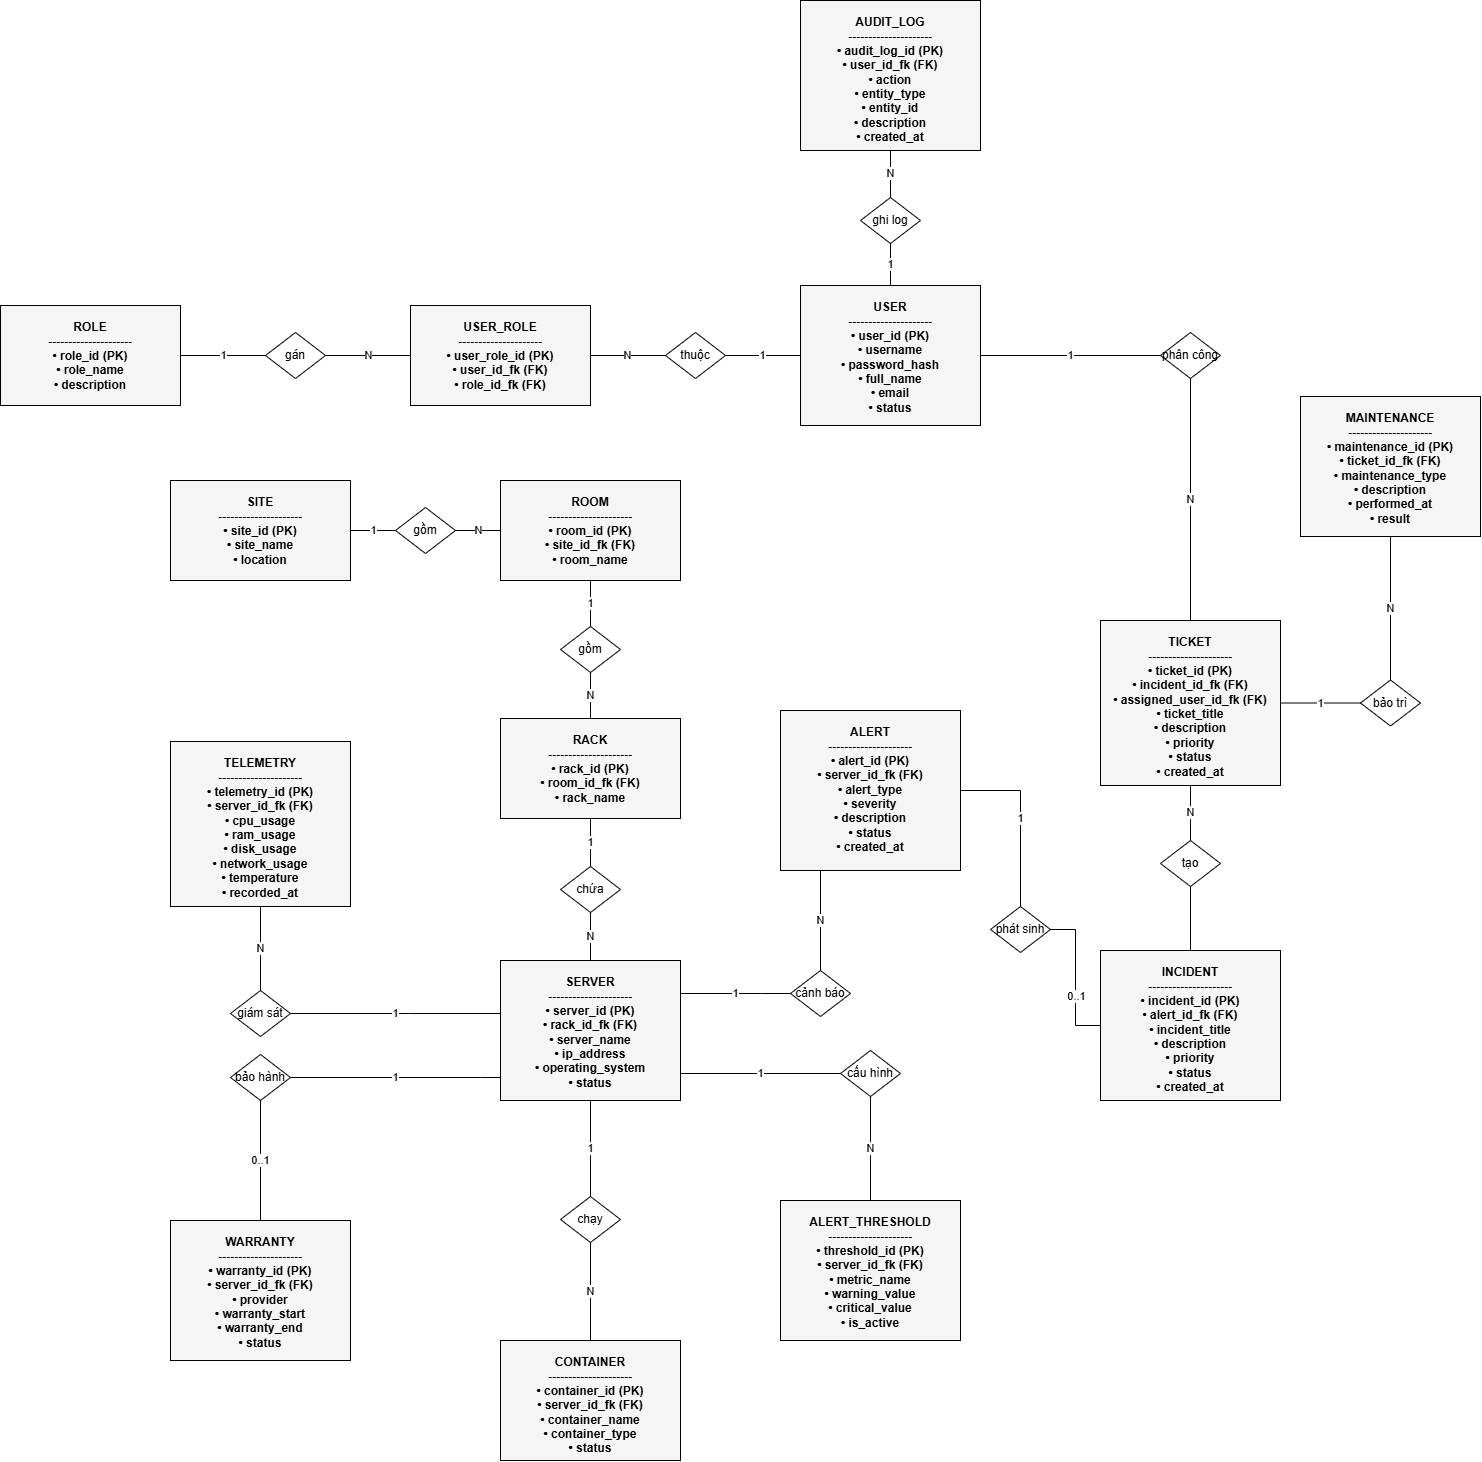
\includegraphics[width=\textwidth,height=0.68\textheight,keepaspectratio]{ERD.drawio.png}
    \caption{Sơ đồ ERD tổng thể của cơ sở dữ liệu AR-IMMS.}
    \label{fig:erd_chuong2}
\end{figure}

\chapter{THIẾT KẾ MỨC LOGIC}

\section{Lược đồ quan hệ}

\begin{itemize}
    \item \textbf{ROLE} (\underline{role\_id}, role\_name, description)
    \item \textbf{USER} (\underline{user\_id}, username, password\_hash, full\_name, email, status)
    \item \textbf{USER\_ROLE} (\underline{user\_role\_id}, user\_id\_fk, role\_id\_fk)
    \item \textbf{SITE} (\underline{site\_id}, site\_name, location)
    \item \textbf{ROOM} (\underline{room\_id}, room\_name, site\_id\_fk)
    \item \textbf{RACK} (\underline{rack\_id}, rack\_name, room\_id\_fk)
    \item \textbf{SERVER} (\underline{server\_id}, server\_name, ip\_address, operating\_system, status, rack\_id\_fk)
    \item \textbf{CONTAINER} (\underline{container\_id}, container\_name, container\_type, status, server\_id\_fk)
    \item \textbf{WARRANTY} (\underline{warranty\_id}, provider, warranty\_start, warranty\_end, status, server\_id\_fk)
    \item \textbf{TELEMETRY} (\underline{telemetry\_id}, cpu\_usage, ram\_usage, disk\_usage, network\_usage, temperature, recorded\_at, server\_id\_fk)
    \item \textbf{ALERT\_THRESHOLD} (\underline{threshold\_id}, metric\_name, warning\_value, critical\_value, is\_active, server\_id\_fk)
    \item \textbf{ALERT} (\underline{alert\_id}, alert\_type, severity, description, status, created\_at, server\_id\_fk)
    \item \textbf{INCIDENT} (\underline{incident\_id}, incident\_title, description, priority, status, created\_at, alert\_id\_fk)
    \item \textbf{TICKET} (\underline{ticket\_id}, ticket\_title, description, priority, status, created\_at, incident\_id\_fk, assigned\_user\_id\_fk)
    \item \textbf{MAINTENANCE} (\underline{maintenance\_id}, maintenance\_type, description, performed\_at, result, ticket\_id\_fk)
    \item \textbf{AUDIT\_LOG} (\underline{audit\_log\_id}, action, entity\_type, entity\_id, description, created\_at, user\_id\_fk)
\end{itemize}

\newpage
\section{Liệt kê khóa chính và khóa ngoại của các thực thể}

\small
\setlength\tabcolsep{4pt}
\begin{longtable}{|c|>{\raggedright\arraybackslash}p{2.8cm}|>{\raggedright\arraybackslash}p{2.6cm}|>{\raggedright\arraybackslash}p{3.1cm}|>{\raggedright\arraybackslash}p{4.2cm}|}
\caption{Danh sách khóa chính và khóa ngoại của các thực thể} \label{tab:pk_fk_c3} \\
\hline
\textbf{STT} & \textbf{Thực thể} & \textbf{Khóa chính (PK)} & \textbf{Khóa ngoại (FK)} & \textbf{Tham chiếu} \\ \hline
\endhead

1 & ROLE & role\_id & -- & -- \\ \hline
2 & USER & user\_id & -- & -- \\ \hline
3 & USER\_ROLE & user\_role\_id & user\_id\_fk \newline role\_id\_fk & USER(user\_id) \newline ROLE(role\_id) \\ \hline
4 & SITE & site\_id & -- & -- \\ \hline
5 & ROOM & room\_id & site\_id\_fk & SITE(site\_id) \\ \hline
6 & RACK & rack\_id & room\_id\_fk & ROOM(room\_id) \\ \hline
7 & SERVER & server\_id & rack\_id\_fk & RACK(rack\_id) \\ \hline
8 & CONTAINER & container\_id & server\_id\_fk & SERVER(server\_id) \\ \hline
9 & WARRANTY & warranty\_id & server\_id\_fk & SERVER(server\_id) \\ \hline
10 & TELEMETRY & telemetry\_id & server\_id\_fk & SERVER(server\_id) \\ \hline
11 & ALERT\_THRESHOLD & threshold\_id & server\_id\_fk & SERVER(server\_id) \\ \hline
12 & ALERT & alert\_id & server\_id\_fk \newline threshold\_id\_fk & SERVER(server\_id) \newline ALERT\_THRESHOLD(threshold\_id) \\ \hline
13 & INCIDENT & incident\_id & alert\_id\_fk & ALERT(alert\_id) \\ \hline
14 & TICKET & ticket\_id & incident\_id\_fk \newline assigned\_user\_id\_fk & INCIDENT(incident\_id) \newline USER(user\_id) \\ \hline
15 & MAINTENANCE & maintenance\_id & ticket\_id\_fk & TICKET(ticket\_id) \\ \hline
16 & AUDIT\_LOG & audit\_log\_id & user\_id\_fk & USER(user\_id) \\ \hline
\end{longtable}

\section{Liệt kê các Constraint của thực thể}

\subsection{ROLE}
\begin{itemize}
    \item \texttt{role\_name}: NOT NULL, UNIQUE.
    \item \texttt{description}: NULL.
\end{itemize}

\subsection{USER}
\begin{itemize}
    \item \texttt{username}: NOT NULL, UNIQUE.
    \item \texttt{password\_hash}: NOT NULL.
    \item \texttt{full\_name}: NOT NULL.
    \item \texttt{email}: NOT NULL, UNIQUE.
    \item \texttt{status}: NOT NULL, DEFAULT 'Inactive'.
\end{itemize}

\subsection{USER\_ROLE}
\begin{itemize}
    \item \texttt{user\_id\_fk}, \texttt{role\_id\_fk}: UNIQUE (Đảm bảo một vai trò không được gán trùng cho cùng một người dùng).
    \item Các cột khóa ngoại (\texttt{user\_id\_fk}, \texttt{role\_id\_fk}): NOT NULL.
\end{itemize}

\subsection{SITE}
\begin{itemize}
    \item \texttt{site\_name}: NOT NULL, UNIQUE.
    \item \texttt{location}: NOT NULL.
\end{itemize}

\subsection{ROOM}
\begin{itemize}
    \item \texttt{room\_name}: NOT NULL.
    \item \texttt{site\_id\_fk}: NOT NULL.
\end{itemize}

\subsection{RACK}
\begin{itemize}
    \item \texttt{rack\_name}: NOT NULL.
    \item \texttt{room\_id\_fk}: NOT NULL.
\end{itemize}

\subsection{SERVER}
\begin{itemize}
    \item \texttt{server\_name}: NOT NULL, UNIQUE.
    \item \texttt{ip\_address}: NOT NULL, UNIQUE.
    \item \texttt{operating\_system}: NOT NULL.
    \item \texttt{status}: NOT NULL, DEFAULT 'Inactive'.
    \item \texttt{rack\_id\_fk}: NOT NULL.
\end{itemize}

\subsection{CONTAINER}
\begin{itemize}
    \item \texttt{container\_name}: NOT NULL.
    \item \texttt{container\_type}: NULL.
    \item \texttt{status}: NOT NULL, DEFAULT 'Inactive'.
    \item \texttt{server\_id\_fk}: NOT NULL.
\end{itemize}

\subsection{WARRANTY}
\begin{itemize}
    \item \texttt{provider}: NOT NULL.
    \item \texttt{warranty\_start}: NOT NULL.
    \item \texttt{warranty\_end}: NOT NULL.
    \item \texttt{status}: NOT NULL.
    \item \texttt{server\_id\_fk}: NOT NULL, UNIQUE.
\end{itemize}

\subsection{TELEMETRY}
\begin{itemize}
    \item \texttt{cpu\_usage}: NOT NULL.
    \item \texttt{ram\_usage}: NOT NULL.
    \item \texttt{disk\_usage}: NOT NULL.
    \item \texttt{network\_usage}: NULL.
    \item \texttt{temperature}: NULL.
    \item \texttt{recorded\_at}: NOT NULL.
    \item \texttt{server\_id\_fk}: NOT NULL.
\end{itemize}

\subsection{ALERT\_THRESHOLD}
\begin{itemize}
    \item \texttt{metric\_name}: NOT NULL.
    \item \texttt{warning\_value}: NOT NULL.
    \item \texttt{critical\_value}: NOT NULL.
    \item \texttt{is\_active}: NOT NULL, DEFAULT 1.
    \item \texttt{server\_id\_fk}: NOT NULL.
\end{itemize}

\subsection{ALERT}
\begin{itemize}
    \item \texttt{alert\_type}: NOT NULL.
    \item \texttt{severity}: NOT NULL.
    \item \texttt{description}: NULL.
    \item \texttt{status}: NOT NULL, DEFAULT 'OPEN'.
    \item \texttt{created\_at}: NOT NULL.
    \item \texttt{server\_id\_fk}: NOT NULL.
\end{itemize}

\subsection{INCIDENT}
\begin{itemize}
    \item \texttt{incident\_title}: NOT NULL.
    \item \texttt{description}: NULL.
    \item \texttt{priority}: NOT NULL.
    \item \texttt{status}: NOT NULL, DEFAULT 'OPEN'.
    \item \texttt{created\_at}: NOT NULL.
    \item \texttt{alert\_id\_fk}: NOT NULL.
\end{itemize}

\subsection{TICKET}
\begin{itemize}
    \item \texttt{ticket\_title}: NOT NULL.
    \item \texttt{description}: NULL.
    \item \texttt{priority}: NOT NULL.
    \item \texttt{status}: NOT NULL, DEFAULT 'OPEN'.
    \item \texttt{created\_at}: NOT NULL.
    \item \texttt{incident\_id\_fk}: NOT NULL.
    \item \texttt{assigned\_user\_id\_fk}: NOT NULL.
\end{itemize}

\subsection{MAINTENANCE}
\begin{itemize}
    \item \texttt{maintenance\_type}: NOT NULL.
    \item \texttt{description}: NULL.
    \item \texttt{performed\_at}: NOT NULL.
    \item \texttt{result}: NULL.
    \item \texttt{ticket\_id\_fk}: NOT NULL.
\end{itemize}

\subsection{AUDIT\_LOG}
\begin{itemize}
    \item \texttt{action}: NOT NULL.
    \item \texttt{entity\_type}: NOT NULL.
    \item \texttt{entity\_id}: NULL.
    \item \texttt{description}: NULL.
    \item \texttt{created\_at}: NOT NULL.
    \item \texttt{user\_id\_fk}: NULL.
\end{itemize}

\section{Chuẩn hóa dữ liệu}

\subsection{Dạng chuẩn thứ nhất (1NF)}
Một quan hệ đạt dạng chuẩn thứ nhất (1NF) khi mỗi thuộc tính chỉ chứa một giá trị nguyên tố, không chứa các nhóm thuộc tính lặp hoặc nhiều giá trị trong cùng một ô.

Trong cơ sở dữ liệu AR-IMMS, các thông tin được tổ chức thành các bảng riêng biệt. Mỗi thuộc tính trong bảng chỉ lưu một giá trị tại một thời điểm.

Ví dụ, thông tin về Server được lưu trong bảng \texttt{SERVER} với các thuộc tính \texttt{server\_id}, \texttt{server\_name}, \texttt{ip\_address}, \texttt{operating\_system} và \texttt{status}. Mỗi thuộc tính chỉ chứa một giá trị tương ứng với từng Server.

\begin{table}[H]
\centering
\caption{Ví dụ minh họa dạng chuẩn 1NF trong bảng SERVER}
\begin{tabular}{|c|c|c|c|c|}
\hline
\textbf{server\_id} & \textbf{server\_name} & \textbf{ip\_address} & \textbf{operating\_system} & \textbf{status} \\ \hline
S001 & Server A & 192.168.1.10 & Linux & Active \\ \hline
S002 & Server B & 192.168.1.11 & Linux & Active \\ \hline
\end{tabular}
\end{table}

Các thông tin có thể phát sinh nhiều bản ghi như Container, Telemetry, Alert và Ticket không được lưu dưới dạng danh sách nhiều giá trị trong bảng \texttt{SERVER} mà được tách thành các bảng riêng biệt. Đối với mối quan hệ nhiều-nhiều giữa \texttt{USER} và \texttt{ROLE}, hệ thống sử dụng bảng trung gian \texttt{USER\_ROLE} thay vì lưu nhiều vai trò trong cùng một thuộc tính của \texttt{USER}.

Do đó, các quan hệ trong cơ sở dữ liệu AR-IMMS đáp ứng yêu cầu của dạng chuẩn thứ nhất (1NF).

\subsection{Dạng chuẩn thứ hai (2NF)}
Một quan hệ đạt dạng chuẩn thứ hai (2NF) khi đã đạt 1NF và mọi thuộc tính không khóa phải phụ thuộc đầy đủ vào toàn bộ khóa chính, không được chỉ phụ thuộc vào một phần của khóa ghép.

Để minh họa, xét quan hệ đăng ký giữa người dùng và vai trò thông qua \texttt{USER\_ROLE}. Khi một quan hệ có khóa ghép gồm \texttt{user\_id} và \texttt{role\_id}, các thuộc tính mô tả riêng User hoặc Role không nên được đặt trực tiếp trong quan hệ này.

Nếu thiết kế không phù hợp như bảng dưới đây, \texttt{user\_name} chỉ phụ thuộc vào \texttt{user\_id} và \texttt{role\_name} chỉ phụ thuộc vào \texttt{role\_id}. Đây là phụ thuộc bộ phận và quan hệ chưa đạt 2NF.

\begin{table}[H]
\centering
\caption{Quan hệ chưa đạt 2NF (chứa phụ thuộc bộ phận)}
\begin{tabular}{|c|c|c|c|}
\hline
\textbf{user\_id} & \textbf{role\_id} & \textbf{user\_name} & \textbf{role\_name} \\ \hline
U001 & R01 & Nguyen Van A & Technician \\ \hline
U001 & R02 & Nguyen Van A & Administrator \\ \hline
U002 & R01 & Tran Van B & Technician \\ \hline
\end{tabular}
\end{table}

Phụ thuộc hàm bị vi phạm:
\begin{itemize}
    \item \texttt{user\_id} $\rightarrow$ \texttt{user\_name}
    \item \texttt{role\_id} $\rightarrow$ \texttt{role\_name}
\end{itemize}

Để loại bỏ phụ thuộc bộ phận, thông tin User và Role được tách khỏi quan hệ \texttt{USER\_ROLE} thành 3 bảng riêng biệt như sau:

\begin{table}[H]
\centering
\caption{Phân tách bảng để đạt dạng chuẩn 2NF}
\begin{subtable}[t]{0.45\textwidth}
\centering
\caption{Bảng USER}
\begin{tabular}{|c|c|}
\hline
\textbf{user\_id} & \textbf{user\_name} \\ \hline
U001 & Nguyen Van A \\ \hline
U002 & Tran Van B \\ \hline
\end{tabular}
\end{subtable}
\hfill
\begin{subtable}[t]{0.45\textwidth}
\centering
\caption{Bảng ROLE}
\begin{tabular}{|c|c|}
\hline
\textbf{role\_id} & \textbf{role\_name} \\ \hline
R01 & Technician \\ \hline
R02 & Administrator \\ \hline
\end{tabular}
\end{subtable}

\vspace{0.3cm}

\begin{subtable}[t]{0.45\textwidth}
\centering
\caption{Bảng USER\_ROLE}
\begin{tabular}{|c|c|}
\hline
\textbf{user\_id} & \textbf{role\_id} \\ \hline
U001 & R01 \\ \hline
U001 & R02 \\ \hline
U002 & R01 \\ \hline
\end{tabular}
\end{subtable}
\end{table}

Sau khi tách, \texttt{USER} quản lý thông tin người dùng, \texttt{ROLE} quản lý thông tin vai trò và \texttt{USER\_ROLE} chỉ quản lý mối quan hệ giữa hai thực thể. Các thuộc tính không khóa không còn phụ thuộc vào một phần của khóa ghép.

Đối với các bảng sử dụng khóa chính đơn như \texttt{USER}, \texttt{ROLE}, \texttt{SERVER}, \texttt{CONTAINER}, \texttt{TELEMETRY}, \texttt{ALERT}, \texttt{INCIDENT}, \texttt{TICKET}, \texttt{MAINTENANCE} và \texttt{AUDIT\_LOG}, không tồn tại phụ thuộc bộ phận vào một phần của khóa. Vì vậy, các quan hệ của AR-IMMS đáp ứng yêu cầu của dạng chuẩn thứ hai (2NF).

\subsection{Dạng chuẩn thứ ba (3NF)}
Một quan hệ đạt dạng chuẩn thứ ba (3NF) khi đã đạt 2NF và không tồn tại phụ thuộc bắc cầu, tức là thuộc tính không khóa không được phụ thuộc vào một thuộc tính không khóa khác.

Trong AR-IMMS, thông tin về hạ tầng được phân tách theo các thực thể Site, Room, Rack và Server. Nếu lưu chung các thông tin này trong một bảng \texttt{SERVER}, có thể phát sinh phụ thuộc bắc cầu:

\begin{table}[H]
\centering
\caption{Ví dụ bảng chứa phụ thuộc bắc cầu (chưa đạt 3NF)}
\begin{tabular}{|c|c|c|c|c|c|}
\hline
\textbf{server\_id} & \textbf{server\_name} & \textbf{rack\_id} & \textbf{rack\_name} & \textbf{room\_id} & \textbf{room\_name} \\ \hline
S001 & Server A & R01 & Rack A & RM01 & Room 1 \\ \hline
S002 & Server B & R01 & Rack A & RM01 & Room 1 \\ \hline
S003 & Server C & R02 & Rack B & RM01 & Room 1 \\ \hline
\end{tabular}
\end{table}

Chuỗi phụ thuộc bắc cầu:
\begin{itemize}
    \item \texttt{server\_id} $\rightarrow$ \texttt{rack\_id} $\rightarrow$ \texttt{rack\_name}
    \item \texttt{rack\_id} $\rightarrow$ \texttt{room\_id} $\rightarrow$ \texttt{room\_name}
\end{itemize}

Trong bảng trên, \texttt{rack\_name} phụ thuộc vào \texttt{rack\_id} thay vì phụ thuộc trực tiếp vào \texttt{server\_id}. Tương tự, \texttt{room\_name} phụ thuộc vào \texttt{room\_id}. Đây là phụ thuộc bắc cầu và làm tăng sự dư thừa dữ liệu.

Để loại bỏ phụ thuộc bắc cầu, thông tin được tách thành các quan hệ tương ứng với từng thực thể:

\begin{table}[H]
\centering
\caption{Phân tách thành các bảng riêng để đạt dạng chuẩn 3NF}
\begin{subtable}[t]{0.45\textwidth}
\centering
\caption{Bảng SERVER}
\begin{tabular}{|c|c|c|}
\hline
\textbf{server\_id} & \textbf{server\_name} & \textbf{rack\_id} \\ \hline
S001 & Server A & R01 \\ \hline
S002 & Server B & R01 \\ \hline
S003 & Server C & R02 \\ \hline
\end{tabular}
\end{subtable}
\hfill
\begin{subtable}[t]{0.45\textwidth}
\centering
\caption{Bảng RACK}
\begin{tabular}{|c|c|c|}
\hline
\textbf{rack\_id} & \textbf{rack\_name} & \textbf{room\_id} \\ \hline
R01 & Rack A & RM01 \\ \hline
R02 & Rack B & RM01 \\ \hline
\end{tabular}
\end{subtable}

\vspace{0.3cm}

\begin{subtable}[t]{0.45\textwidth}
\centering
\caption{Bảng ROOM}
\begin{tabular}{|c|c|c|}
\hline
\textbf{room\_id} & \textbf{room\_name} & \textbf{site\_id} \\ \hline
RM01 & Room 1 & ST01 \\ \hline
\end{tabular}
\end{subtable}
\hfill
\begin{subtable}[t]{0.45\textwidth}
\centering
\caption{Bảng SITE}
\begin{tabular}{|c|c|}
\hline
\textbf{site\_id} & \textbf{site\_name} \\ \hline
ST01 & Main Site \\ \hline
\end{tabular}
\end{subtable}
\end{table}

Sau khi tách, thông tin Server chỉ phụ thuộc vào \texttt{server\_id}, thông tin Rack phụ thuộc vào \texttt{rack\_id}, thông tin Room phụ thuộc vào \texttt{room\_id} và thông tin Site phụ thuộc vào \texttt{site\_id}. Do đó, phụ thuộc bắc cầu được loại bỏ hoàn toàn.

Tương tự, các thông tin về User, Role, Container, Telemetry, Alert, Incident, Ticket và Maintenance được tổ chức thành các quan hệ riêng biệt theo đúng thực thể mà chúng mô tả.

Do các thuộc tính được tổ chức theo đúng thực thể và không tồn tại phụ thuộc bắc cầu trong cùng một quan hệ theo mô hình đã xác định, các quan hệ của AR-IMMS đáp ứng yêu cầu của dạng chuẩn thứ ba (3NF).

\subsection{Dạng chuẩn Boyce--Codd (BCNF) và Phụ thuộc hàm}
Để hạn chế dư thừa dữ liệu và tránh các bất thường khi thao tác dữ liệu, các quan hệ trong cơ sở dữ liệu AR-IMMS được kiểm tra dựa trên các phụ thuộc hàm và các ràng buộc khóa đã xác định.

Một quan hệ đạt dạng chuẩn Boyce–Codd (BCNF) khi với mọi phụ thuộc hàm phi tầm thường X → Y được xác định trên quan hệ, X phải là một siêu khóa (Superkey) của quan hệ đó.

Dựa trên các khóa chính (PK), khóa ứng viên được tạo từ các ràng buộc UNIQUE và cấu trúc thuộc tính của các bảng, các phụ thuộc hàm chính của hệ thống được xác định như sau:

{\small
\textbf{1. Nhóm thực thể phân quyền và người dùng}
\begin{itemize}
    \item \textbf{ROLE:}
    \begin{itemize}
        \item \texttt{role\_id} $\rightarrow$ \texttt{\{role\_name, description\}}
        \item \texttt{role\_name} $\rightarrow$ \texttt{\{role\_id, description\}} (Do \texttt{role\_name} là UNIQUE)
    \end{itemize}
    \item \textbf{USER:}
    \begin{itemize}
        \item \texttt{user\_id} $\rightarrow$ \texttt{\{username, password\_hash, full\_name, email, status\}}
        \item \texttt{username} $\rightarrow$ \texttt{\{user\_id, password\_hash, full\_name, email, status\}} (Do \texttt{username} là UNIQUE)
        \item \texttt{email} $\rightarrow$ \texttt{\{user\_id, username, password\_hash, full\_name, status\}} (Do \texttt{email} là UNIQUE)
    \end{itemize}
    \item \textbf{USER\_ROLE:}
    \begin{itemize}
        \item \texttt{user\_role\_id} $\rightarrow$ \texttt{\{user\_id\_fk, role\_id\_fk\}}
        \item \texttt{(user\_id\_fk, role\_id\_fk)} $\rightarrow$ \texttt{user\_role\_id} (Do khóa ghép UNIQUE)
    \end{itemize}
\end{itemize}

\textbf{2. Nhóm thực thể hạ tầng (Infrastructure)}
\begin{itemize}
    \item \textbf{SITE:}
    \begin{itemize}
        \item \texttt{site\_id} $\rightarrow$ \texttt{\{site\_name, location\}}
        \item \texttt{site\_name} $\rightarrow$ \texttt{\{site\_id, location\}} (Do \texttt{site\_name} là UNIQUE)
    \end{itemize}
    \item \textbf{ROOM:}
    \begin{itemize}
        \item \texttt{room\_id} $\rightarrow$ \texttt{\{room\_name, site\_id\_fk\}}
    \end{itemize}
    \item \textbf{RACK:}
    \begin{itemize}
        \item \texttt{rack\_id} $\rightarrow$ \texttt{\{rack\_name, room\_id\_fk\}}
    \end{itemize}
    \item \textbf{SERVER:}
    \begin{itemize}
        \item \texttt{server\_id} $\rightarrow$ \texttt{\{server\_name, ip\_address, operating\_system, status, rack\_id\_fk\}}
        \item \texttt{server\_name} $\rightarrow$ \texttt{\{server\_id, ip\_address, operating\_system, status, rack\_id\_fk\}} (Do UNIQUE)
        \item \texttt{ip\_address} $\rightarrow$ \texttt{\{server\_id, server\_name, operating\_system, status, rack\_id\_fk\}} (Do UNIQUE)
    \end{itemize}
\end{itemize}

\textbf{3. Nhóm thực thể tài nguyên và cấu hình}
\begin{itemize}
    \item \textbf{CONTAINER:}
    \begin{itemize}
        \item \texttt{container\_id} $\rightarrow$ \texttt{\{container\_name, container\_type, status, server\_id\_fk\}}
    \end{itemize}
    \item \textbf{WARRANTY:}
    \begin{itemize}
        \item \texttt{warranty\_id} $\rightarrow$ \texttt{\{provider, warranty\_start, warranty\_end, status, server\_id\_fk\}}
        \item \texttt{server\_id\_fk} $\rightarrow$ \texttt{\{warranty\_id, provider, warranty\_start, warranty\_end, status\}} (Do UNIQUE)
    \end{itemize}
    \item \textbf{ALERT\_THRESHOLD:}
    \begin{itemize}
        \item \texttt{threshold\_id} $\rightarrow$ \texttt{\{metric\_name, warning\_value, critical\_value, is\_active, server\_id\_fk\}}
    \end{itemize}
\end{itemize}

\textbf{4. Nhóm thực thể giám sát và sự cố (Monitoring \& Operations)}
\begin{itemize}
    \item \textbf{TELEMETRY:}
    \begin{itemize}
        \item \texttt{telemetry\_id} $\rightarrow$ \texttt{\{cpu\_usage, ram\_usage, disk\_usage, network\_usage, temperature, recorded\_at, server\_id\_fk\}}
    \end{itemize}
    \item \textbf{ALERT:}
    \begin{itemize}
        \item \texttt{alert\_id} $\rightarrow$ \texttt{\{alert\_type, severity, description, status, created\_at, server\_id\_fk\}}
    \end{itemize}
    \item \textbf{INCIDENT:}
    \begin{itemize}
        \item \texttt{incident\_id} $\rightarrow$ \texttt{\{incident\_title, description, priority, status, created\_at, alert\_id\_fk\}}
    \end{itemize}
    \item \textbf{TICKET:}
    \begin{itemize}
        \item \texttt{ticket\_id} $\rightarrow$ \texttt{\{ticket\_title, description, priority, status, created\_at, incident\_id\_fk, assigned\_user\_id\_fk\}}
    \end{itemize}
    \item \textbf{MAINTENANCE:}
    \begin{itemize}
        \item \texttt{maintenance\_id} $\rightarrow$ \texttt{\{maintenance\_type, description, performed\_at, result, ticket\_id\_fk\}}
    \end{itemize}
    \item \textbf{AUDIT\_LOG:}
    \begin{itemize}
        \item \texttt{audit\_log\_id} $\rightarrow$ \texttt{\{action, entity\_type, entity\_id, description, created\_at, user\_id\_fk\}}
    \end{itemize}
\end{itemize}
} % hết \small

\subsubsection*{Kết luận}

Đối với các phụ thuộc hàm được xác định ở trên, vế trái của mỗi phụ thuộc hàm phi tầm thường đều là khóa chính hoặc khóa ứng viên, do đó đều là siêu khóa của quan hệ tương ứng. Vì vậy, các quan hệ trong cơ sở dữ liệu AR-IMMS đáp ứng điều kiện của dạng chuẩn Boyce–Codd (BCNF) dựa trên các phụ thuộc hàm và ràng buộc khóa đã được xác định.

\subsection{Tổng hợp kết quả chuẩn hóa}

\begin{table}[H]
\centering
\caption{Tổng hợp kết quả đánh giá các dạng chuẩn của cơ sở dữ liệu AR-IMMS}
\begin{tabular}{|c|l|c|c|c|c|}
\hline
\textbf{STT} & \textbf{Bảng (Thực thể)} & \textbf{1NF} & \textbf{2NF} & \textbf{3NF} & \textbf{BCNF} \\ \hline
1 & USER & Đạt & Đạt & Đạt & Đạt \\ \hline
2 & ROLE & Đạt & Đạt & Đạt & Đạt \\ \hline
3 & USER\_ROLE & Đạt & Đạt & Đạt & Đạt \\ \hline
4 & SITE & Đạt & Đạt & Đạt & Đạt \\ \hline
5 & ROOM & Đạt & Đạt & Đạt & Đạt \\ \hline
6 & RACK & Đạt & Đạt & Đạt & Đạt \\ \hline
7 & SERVER & Đạt & Đạt & Đạt & Đạt \\ \hline
8 & CONTAINER & Đạt & Đạt & Đạt & Đạt \\ \hline
9 & WARRANTY & Đạt & Đạt & Đạt & Đạt \\ \hline
10 & TELEMETRY & Đạt & Đạt & Đạt & Đạt \\ \hline
11 & ALERT\_THRESHOLD & Đạt & Đạt & Đạt & Đạt \\ \hline
12 & ALERT & Đạt & Đạt & Đạt & Đạt \\ \hline
13 & INCIDENT & Đạt & Đạt & Đạt & Đạt \\ \hline
14 & TICKET & Đạt & Đạt & Đạt & Đạt \\ \hline
15 & MAINTENANCE & Đạt & Đạt & Đạt & Đạt \\ \hline
16 & AUDIT\_LOG & Đạt & Đạt & Đạt & Đạt \\ \hline
\end{tabular}
\end{table}

Qua quá trình kiểm tra các dạng chuẩn từ 1NF, 2NF, 3NF đến BCNF, cơ sở dữ liệu AR-IMMS được tổ chức thành các quan hệ riêng biệt, trong đó các thuộc tính được phân bổ theo đúng thực thể và được liên kết thông qua khóa chính, khóa ngoại. Thiết kế này giúp giảm sự dư thừa dữ liệu, hạn chế các bất thường khi thao tác dữ liệu và đảm bảo tính nhất quán của cơ sở dữ liệu.

Theo các phụ thuộc hàm được xác định trong mô hình, các quan hệ của cơ sở dữ liệu AR-IMMS đạt đến BCNF.

\chapter{THIẾT KẾ MỨC VẬT LÍ}
\label{chap:trien_khai_csdl}

\section{XÁC ĐỊNH HỆ QUẢN TRỊ CƠ SỞ DỮ LIỆU}
Nhóm lựa chọn Microsoft SQL Server (Express/Developer Edition) làm hệ quản trị cơ sở dữ liệu (DBMS) để triển khai hệ thống AR\_IMMS dựa trên các lý do kỹ thuật và thực tiễn sau:

\begin{itemize}
    \item \textbf{Chi phí và Quy mô:} Miễn phí bản quyền sử dụng, hoàn toàn đủ khả năng đáp ứng quy mô đồ án với 16 thực thể dữ liệu.
    \item \textbf{Ràng buộc toàn vẹn:} Hỗ trợ đầy đủ và chặt chẽ các ràng buộc toàn vẹn dữ liệu như PRIMARY KEY, FOREIGN KEY, NOT NULL, UNIQUE, DEFAULT, và CHECK.
    \item \textbf{Công cụ quản lý:} Hỗ trợ công cụ quản lý trực quan SQL Server Management Studio (SSMS) giúp dễ dàng trong việc thiết kế, khởi tạo, viết truy vấn và kiểm thử dữ liệu.
    \item \textbf{Kiểu dữ liệu phù hợp:} Hỗ trợ tốt kiểu dữ liệu ngày giờ (DATETIME), đặc biệt phù hợp với nhóm dữ liệu TELEMETRY (dữ liệu chuỗi thời gian - time-series data).
    \item \textbf{Khả năng mở rộng:} Ngôn ngữ T-SQL mạnh mẽ, hỗ trợ tốt các thao tác nâng cao như JOIN, VIEW, STORED PROCEDURE, và TRIGGER nhằm phục vụ cho việc phát triển và mở rộng các nghiệp vụ phức tạp sau này.
\end{itemize}

\section{TẠO DATABASE AR\_IMMS}
Để triển khai hệ thống quản lý cơ sở dữ liệu AR-IMMS, nhóm sử dụng SQL Server làm hệ quản trị cơ sở dữ liệu. Cơ sở dữ liệu AR\_IMMS được khởi tạo nhằm lưu trữ và quản lý toàn bộ dữ liệu phục vụ cho hoạt động vận hành của hệ thống.

Database được khởi tạo bằng câu lệnh T-SQL sau:

\begin{lstlisting}[language=SQL]
CREATE DATABASE AR_IMMS;
GO
\end{lstlisting}

Hình ảnh minh họa việc khởi tạo Database trong SQL Server Management Studio (SSMS):

\begin{figure}[H]
    \centering
    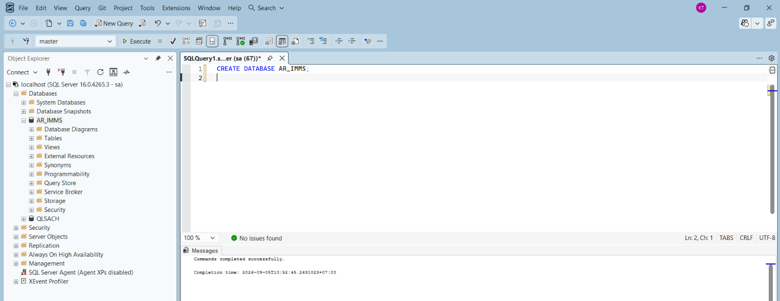
\includegraphics[width=0.95\textwidth]{imagesssms_create_db.png} % Thay duong dan anh cua ban
    \caption{Khởi tạo Database AR\_IMMS trong SSMS}
    \label{fig:create_db}
\end{figure}

\section{VIẾT LỆNH TẠO BẢNG}
\noindent \textbf{Hệ quản trị cơ sở dữ liệu:} SQL Server

\begin{lstlisting}[language=SQL]
-- 1. Bang ROLE
CREATE TABLE [ROLE] (
    role_id INT IDENTITY(1,1) PRIMARY KEY,
    role_name NVARCHAR(100) NOT NULL,
    description NVARCHAR(255) NULL
);

-- 2. Bang USER
CREATE TABLE [USER] (
    user_id INT IDENTITY(1,1) PRIMARY KEY,
    username VARCHAR(50) NOT NULL,
    password_hash VARCHAR(255) NOT NULL,
    full_name NVARCHAR(100) NOT NULL,
    email VARCHAR(100) NOT NULL,
    status VARCHAR(20) NOT NULL
);

-- 3. Bang USER_ROLE
CREATE TABLE [USER_ROLE] (
    user_role_id INT IDENTITY(1,1) PRIMARY KEY,
    user_id_fk INT NOT NULL,
    role_id_fk INT NOT NULL
);

-- 4. Bang SITE
CREATE TABLE [SITE] (
    site_id INT IDENTITY(1,1) PRIMARY KEY,
    site_name NVARCHAR(100) NOT NULL,
    location NVARCHAR(255) NOT NULL
);

-- 5. Bang ROOM
CREATE TABLE [ROOM] (
    room_id INT IDENTITY(1,1) PRIMARY KEY,
    room_name NVARCHAR(100) NOT NULL,
    site_id_fk INT NOT NULL
);

-- 6. Bang RACK
CREATE TABLE [RACK] (
    rack_id INT IDENTITY(1,1) PRIMARY KEY,
    rack_name NVARCHAR(100) NOT NULL,
    room_id_fk INT NOT NULL
);

-- 7. Bang SERVER
CREATE TABLE [SERVER] (
    server_id INT IDENTITY(1,1) PRIMARY KEY,
    server_name NVARCHAR(100) NOT NULL,
    ip_address VARCHAR(15) NOT NULL,
    operating_system NVARCHAR(100) NOT NULL,
    status VARCHAR(20) NOT NULL,
    rack_id_fk INT NOT NULL
);

-- 8. Bang CONTAINER
CREATE TABLE [CONTAINER] (
    container_id INT IDENTITY(1,1) PRIMARY KEY,
    container_name NVARCHAR(100) NOT NULL,
    container_type NVARCHAR(50) NULL,
    status VARCHAR(20) NOT NULL,
    server_id_fk INT NOT NULL
);

-- 9. Bang WARRANTY
CREATE TABLE [WARRANTY] (
    warranty_id INT IDENTITY(1,1) PRIMARY KEY,
    provider NVARCHAR(100) NOT NULL,
    warranty_start DATE NOT NULL,
    warranty_end DATE NOT NULL,
    status NVARCHAR(50) NOT NULL,
    server_id_fk INT NOT NULL
);

-- 10. Bang TELEMETRY
CREATE TABLE [TELEMETRY] (
    telemetry_id INT IDENTITY(1,1) PRIMARY KEY,
    cpu_usage FLOAT NOT NULL,
    ram_usage FLOAT NOT NULL,
    disk_usage FLOAT NOT NULL,
    network_usage FLOAT NULL,
    temperature FLOAT NULL,
    recorded_at DATETIME NOT NULL,
    server_id_fk INT NOT NULL
);

-- 11. Bang ALERT_THRESHOLD
CREATE TABLE [ALERT_THRESHOLD] (
    threshold_id INT IDENTITY(1,1) PRIMARY KEY,
    metric_name VARCHAR(50) NOT NULL,
    warning_value FLOAT NOT NULL,
    critical_value FLOAT NOT NULL,
    is_active BIT NOT NULL,
    server_id_fk INT NOT NULL
);

-- 12. Bang ALERT
CREATE TABLE [ALERT] (
    alert_id INT IDENTITY(1,1) PRIMARY KEY,
    alert_type VARCHAR(50) NOT NULL,
    severity VARCHAR(20) NOT NULL,
    description NVARCHAR(MAX) NULL,
    status VARCHAR(20) NOT NULL,
    created_at DATETIME NOT NULL,
    server_id_fk INT NOT NULL
);

-- 13. Bang INCIDENT
CREATE TABLE [INCIDENT] (
    incident_id INT IDENTITY(1,1) PRIMARY KEY,
    incident_title NVARCHAR(200) NOT NULL,
    description NVARCHAR(MAX) NULL,
    priority VARCHAR(20) NOT NULL,
    status VARCHAR(20) NOT NULL,
    created_at DATETIME NOT NULL,
    alert_id_fk INT NOT NULL
);

-- 14. Bang TICKET
CREATE TABLE [TICKET] (
    ticket_id INT IDENTITY(1,1) PRIMARY KEY,
    ticket_title NVARCHAR(200) NOT NULL,
    description NVARCHAR(MAX) NULL,
    priority VARCHAR(20) NOT NULL,
    status VARCHAR(20) NOT NULL,
    created_at DATETIME NOT NULL,
    incident_id_fk INT NOT NULL,
    assigned_user_id_fk INT NOT NULL
);

-- 15. Bang MAINTENANCE
CREATE TABLE [MAINTENANCE] (
    maintenance_id INT IDENTITY(1,1) PRIMARY KEY,
    maintenance_type NVARCHAR(100) NOT NULL,
    description NVARCHAR(MAX) NULL,
    performed_at DATETIME NOT NULL,
    result NVARCHAR(MAX) NULL,
    ticket_id_fk INT NOT NULL
);

-- 16. Bang AUDIT_LOG
CREATE TABLE [AUDIT_LOG] (
    audit_log_id INT IDENTITY(1,1) PRIMARY KEY,
    action NVARCHAR(200) NOT NULL,
    entity_type VARCHAR(50) NOT NULL,
    entity_id INT NULL,
    description NVARCHAR(MAX) NULL,
    created_at DATETIME NOT NULL,
    user_id_fk INT NULL
);
\end{lstlisting}

\section{THIẾT LẬP CONSTRAINT}
\noindent \textbf{Hệ quản trị:} SQL Server

\subsection{FOREIGN KEY}
\begin{lstlisting}[language=SQL]
USE AR_IMMS;
GO

-- USER_ROLE
ALTER TABLE [USER_ROLE]
ADD CONSTRAINT FK_USER_ROLE_USER
FOREIGN KEY (user_id_fk) REFERENCES [USER](user_id);

ALTER TABLE [USER_ROLE]
ADD CONSTRAINT FK_USER_ROLE_ROLE
FOREIGN KEY (role_id_fk) REFERENCES [ROLE](role_id);

-- ROOM
ALTER TABLE [ROOM]
ADD CONSTRAINT FK_ROOM_SITE
FOREIGN KEY (site_id_fk) REFERENCES [SITE](site_id);

-- RACK
ALTER TABLE [RACK]
ADD CONSTRAINT FK_RACK_ROOM
FOREIGN KEY (room_id_fk) REFERENCES [ROOM](room_id);

-- SERVER
ALTER TABLE [SERVER]
ADD CONSTRAINT FK_SERVER_RACK
FOREIGN KEY (rack_id_fk) REFERENCES [RACK](rack_id);

-- CONTAINER
ALTER TABLE [CONTAINER]
ADD CONSTRAINT FK_CONTAINER_SERVER
FOREIGN KEY (server_id_fk) REFERENCES [SERVER](server_id);

-- WARRANTY
ALTER TABLE [WARRANTY]
ADD CONSTRAINT FK_WARRANTY_SERVER
FOREIGN KEY (server_id_fk) REFERENCES [SERVER](server_id);

-- TELEMETRY (Da sua tham chieu thanh server_id)
ALTER TABLE [TELEMETRY]
ADD CONSTRAINT FK_TELEMETRY_SERVER
FOREIGN KEY (server_id_fk) REFERENCES [SERVER](server_id);

-- ALERT_THRESHOLD (Da sua tham chieu thanh server_id)
ALTER TABLE [ALERT_THRESHOLD]
ADD CONSTRAINT FK_ALERT_THRESHOLD_SERVER
FOREIGN KEY (server_id_fk) REFERENCES [SERVER](server_id);

-- ALERT (Da sua tham chieu thanh server_id)
ALTER TABLE [ALERT]
ADD CONSTRAINT FK_ALERT_SERVER
FOREIGN KEY (server_id_fk) REFERENCES [SERVER](server_id);

-- INCIDENT
ALTER TABLE [INCIDENT]
ADD CONSTRAINT FK_INCIDENT_ALERT
FOREIGN KEY (alert_id_fk) REFERENCES [ALERT](alert_id);

-- TICKET
ALTER TABLE [TICKET]
ADD CONSTRAINT FK_TICKET_INCIDENT
FOREIGN KEY (incident_id_fk) REFERENCES [INCIDENT](incident_id);

ALTER TABLE [TICKET]
ADD CONSTRAINT FK_TICKET_ASSIGNED_USER
FOREIGN KEY (assigned_user_id_fk) REFERENCES [USER](user_id);

-- MAINTENANCE
ALTER TABLE [MAINTENANCE]
ADD CONSTRAINT FK_MAINTENANCE_TICKET
FOREIGN KEY (ticket_id_fk) REFERENCES [TICKET](ticket_id);

-- AUDIT_LOG
ALTER TABLE [AUDIT_LOG]
ADD CONSTRAINT FK_AUDIT_LOG_USER
FOREIGN KEY (user_id_fk) REFERENCES [USER](user_id);
GO
\end{lstlisting}

\subsection{UNIQUE CONSTRAINT}
\begin{lstlisting}[language=SQL]
USE AR_IMMS;
GO

ALTER TABLE [ROLE]
ADD CONSTRAINT UQ_ROLE_NAME UNIQUE (role_name);

ALTER TABLE [USER]
ADD CONSTRAINT UQ_USER_USERNAME UNIQUE (username);

ALTER TABLE [USER]
ADD CONSTRAINT UQ_USER_EMAIL UNIQUE (email);

ALTER TABLE [USER_ROLE]
ADD CONSTRAINT UQ_USER_ROLE UNIQUE (user_id_fk, role_id_fk);

ALTER TABLE [SITE]
ADD CONSTRAINT UQ_SITE_NAME UNIQUE (site_name);

-- SERVER (Bo sung UNIQUE cho server_name va ip_address)
ALTER TABLE [SERVER]
ADD CONSTRAINT UQ_SERVER_NAME UNIQUE (server_name);

ALTER TABLE [SERVER]
ADD CONSTRAINT UQ_SERVER_IP UNIQUE (ip_address);

-- WARRANTY
ALTER TABLE [WARRANTY]
ADD CONSTRAINT UQ_WARRANTY_SERVER UNIQUE (server_id_fk);

-- ALERT_THRESHOLD
ALTER TABLE [ALERT_THRESHOLD]
ADD CONSTRAINT UQ_ALERT_THRESHOLD UNIQUE (server_id_fk, metric_name);
GO
\end{lstlisting}

\subsection{CHECK CONSTRAINT}
\begin{lstlisting}[language=SQL]
USE AR_IMMS;
GO

-- USER
ALTER TABLE [USER]
ADD CONSTRAINT CK_USER_STATUS
CHECK (status IN ('ACTIVE', 'INACTIVE'));

-- SERVER
ALTER TABLE [SERVER]
ADD CONSTRAINT CK_SERVER_STATUS
CHECK (status IN ('ONLINE', 'OFFLINE', 'MAINTENANCE', 'INACTIVE'));

-- CONTAINER
ALTER TABLE [CONTAINER]
ADD CONSTRAINT CK_CONTAINER_STATUS
CHECK (status IN ('RUNNING', 'STOPPED', 'PAUSED', 'INACTIVE'));

-- WARRANTY
ALTER TABLE [WARRANTY]
ADD CONSTRAINT CK_WARRANTY_DATE
CHECK (warranty_end >= warranty_start);

-- TELEMETRY
ALTER TABLE [TELEMETRY]
ADD CONSTRAINT CK_TELEMETRY_CPU
CHECK (cpu_usage >= 0 AND cpu_usage <= 100);

ALTER TABLE [TELEMETRY]
ADD CONSTRAINT CK_TELEMETRY_RAM
CHECK (ram_usage >= 0 AND ram_usage <= 100);

ALTER TABLE [TELEMETRY]
ADD CONSTRAINT CK_TELEMETRY_DISK
CHECK (disk_usage >= 0 AND disk_usage <= 100);

-- ALERT_THRESHOLD
ALTER TABLE [ALERT_THRESHOLD]
ADD CONSTRAINT CK_THRESHOLD_VALUES
CHECK (warning_value >= 0 AND critical_value >= warning_value);

-- ALERT
ALTER TABLE [ALERT]
ADD CONSTRAINT CK_ALERT_SEVERITY
CHECK (severity IN ('WARNING', 'CRITICAL'));

ALTER TABLE [ALERT]
ADD CONSTRAINT CK_ALERT_STATUS
CHECK (status IN ('OPEN', 'ACKNOWLEDGED', 'RESOLVED', 'CLOSED'));

-- INCIDENT
ALTER TABLE [INCIDENT]
ADD CONSTRAINT CK_INCIDENT_PRIORITY
CHECK (priority IN ('LOW', 'MEDIUM', 'HIGH', 'CRITICAL'));

ALTER TABLE [INCIDENT]
ADD CONSTRAINT CK_INCIDENT_STATUS
CHECK (status IN ('OPEN', 'IN_PROGRESS', 'RESOLVED', 'CLOSED'));

-- TICKET
ALTER TABLE [TICKET]
ADD CONSTRAINT CK_TICKET_PRIORITY
CHECK (priority IN ('LOW', 'MEDIUM', 'HIGH', 'CRITICAL'));

ALTER TABLE [TICKET]
ADD CONSTRAINT CK_TICKET_STATUS
CHECK (status IN ('OPEN', 'IN_PROGRESS', 'RESOLVED', 'CLOSED'));
GO
\end{lstlisting}

\subsection{DEFAULT CONSTRAINT}
\begin{lstlisting}[language=SQL]
USE AR_IMMS;
GO

ALTER TABLE [USER]
ADD CONSTRAINT DF_USER_STATUS DEFAULT 'Inactive' FOR status;

ALTER TABLE [SERVER]
ADD CONSTRAINT DF_SERVER_STATUS DEFAULT 'Inactive' FOR status;

ALTER TABLE [CONTAINER]
ADD CONSTRAINT DF_CONTAINER_STATUS DEFAULT 'Inactive' FOR status;

ALTER TABLE [ALERT_THRESHOLD]
ADD CONSTRAINT DF_ALERT_THRESHOLD_ACTIVE DEFAULT 1 FOR is_active;

ALTER TABLE [ALERT]
ADD CONSTRAINT DF_ALERT_STATUS DEFAULT 'OPEN' FOR status;

ALTER TABLE [ALERT]
ADD CONSTRAINT DF_ALERT_CREATED_AT DEFAULT GETDATE() FOR created_at;

ALTER TABLE [INCIDENT]
ADD CONSTRAINT DF_INCIDENT_STATUS DEFAULT 'OPEN' FOR status;

ALTER TABLE [INCIDENT]
ADD CONSTRAINT DF_INCIDENT_CREATED_AT DEFAULT GETDATE() FOR created_at;

ALTER TABLE [TICKET]
ADD CONSTRAINT DF_TICKET_STATUS DEFAULT 'OPEN' FOR status;

ALTER TABLE [TICKET]
ADD CONSTRAINT DF_TICKET_CREATED_AT DEFAULT GETDATE() FOR created_at;

ALTER TABLE [MAINTENANCE]
ADD CONSTRAINT DF_MAINTENANCE_PERFORMED_AT DEFAULT GETDATE() FOR performed_at;

ALTER TABLE [AUDIT_LOG]
ADD CONSTRAINT DF_AUDIT_LOG_CREATED_AT DEFAULT GETDATE() FOR created_at;
GO
\end{lstlisting}

\section{CHÈN DỮ LIỆU}
Dữ liệu mẫu của nhóm được sử dụng để kiểm thử cơ sở dữ liệu được tạo bằng công cụ Mockaroo. Dữ liệu được xây dựng dựa trên cấu trúc 16 bảng, các thuộc tính và mối quan hệ đã thiết kế ở các chương trước. Sau khi tạo, dữ liệu được kiểm tra và điều chỉnh để đảm bảo tính hợp lệ của các khóa chính, khóa ngoại và các ràng buộc trong cơ sở dữ liệu. 

\vspace{0.5em}
\noindent \textbf{THỨ TỰ NHẬP DỮ LIỆU CHO DATABASE AR\_IMMS}

\subsection{QUẢN LÝ NGƯỜI DÙNG \& PHÂN QUYỀN (USER -- ROLE -- USER\_ROLE)}

\paragraph{a. Bảng ROLE (Vai trò / Nhóm quyền)}
\begin{itemize}
    \item \textbf{Mục đích:} Khởi tạo danh mục nhóm quyền (Admin, Operator, Technician).
    \item \textbf{Lý do nạp trước:} Là bảng danh mục chuẩn hóa độc lập, không phụ thuộc vào các bảng khác.
\end{itemize}

\paragraph{b. Bảng USER (Tài khoản người dùng)}
\begin{itemize}
    \item \textbf{Mục đích:} Lưu thông tin cá nhân và tài khoản đăng nhập của nhân viên.
    \item \textbf{Lý do nạp trước USER\_ROLE:} Cần tạo danh sách tài khoản người dùng trước để có \texttt{user\_id} tham chiếu.
\end{itemize}

\paragraph{c. Bảng USER\_ROLE (Phân quyền tài khoản)}
\begin{itemize}
    \item \textbf{Mục đích:} Gán vai trò/quyền hạn cụ thể cho từng tài khoản.
    \item \textbf{Lý do nạp cuối Phần 2:} Bảng này đóng vai trò giải quyết mối quan hệ Nhiều - Nhiều (N-N), bắt buộc phải có sẵn cả \texttt{user\_id\_fk} và \texttt{role\_id\_fk} từ hai bảng trên mới có thể thực hiện liên kết.
\end{itemize}

\subsection{HẠ TẦNG VẬT LÝ \& THU THẬP DỮ LIỆU (SITE -- ROOM -- RACK -- SERVER -- TELEMETRY)}

\paragraph{a. Bảng SITE (Trung tâm dữ liệu)}
\begin{itemize}
    \item \textbf{Mục đích:} Lưu thông tin các vị trí trung tâm dữ liệu vật lý (Hà Nội, TP.HCM, Đà Nẵng).
    \item \textbf{Lý do nạp trước:} Đây là thực thể gốc cấp cao nhất trong hệ thống hạ tầng, độc lập và không chứa bất kỳ khóa ngoại (FK) nào.
\end{itemize}

\paragraph{b. Bảng ROOM (Phòng máy chủ)}
\begin{itemize}
    \item \textbf{Mục đích:} Lưu trữ danh sách các phòng máy chủ thuộc từng trung tâm dữ liệu.
    \item \textbf{Lý do nạp sau SITE:} Mỗi phòng máy bắt buộc phải thuộc một Site xác định thông qua \texttt{site\_id\_fk}. Cần có dữ liệu SITE trước để lấy ID tham chiếu hợp lệ.
\end{itemize}

\paragraph{c. Bảng RACK (Tủ Rack)}
\begin{itemize}
    \item \textbf{Mục đích:} Quản lý vị trí các tủ đĩa/tủ chứa thiết bị trong phòng máy.
    \item \textbf{Lý do nạp sau ROOM:} Mỗi tủ Rack phải được định vị bên trong một phòng máy cụ thể thông qua \texttt{room\_id\_fk}.
\end{itemize}

\paragraph{d. Bảng SERVER (Máy chủ vật lý)}
\noindent Ở bảng SERVER sẽ đc lấy dữ liệu từ file csv (\url{https://drive.google.com/file/d/1gjNlxpAloXAcxYxCO2b5VRABCf3k2lhI/view?usp=sharing})
\begin{itemize}
    \item \textbf{Mục đích:} Định danh máy chủ, lưu thông tin cấu hình phần cứng và vị trí lắp đặt.
    \item \textbf{Lý do nạp sau RACK:} Máy chủ vật lý phải được gán cố định vào một tủ Rack xác định thông qua \texttt{rack\_id\_fk}.
\end{itemize}

\paragraph{e. Bảng TELEMETRY (Dữ liệu giám sát cảm biến)}
\noindent Ở bảng TELEMETRY sẽ đc lấy dữ liệu từ file csv (\url{https://drive.google.com/file/d/1gjNlxpAloXAcxYxCO2b5VRABCf3k2lhI/view?usp=sharing})
\begin{itemize}
    \item \textbf{Mục đích:} Lưu các chỉ số vận hành thu thập theo thời gian thực (CPU, RAM, Nhiệt độ).
    \item \textbf{Lý do nạp sau SERVER:} Dữ liệu cảm biến không thể tồn tại độc lập mà bắt buộc phải gắn với một máy chủ cụ thể thông qua \texttt{server\_id\_fk}.
\end{itemize}

\subsection{Môi trường ảo và thông tin bảo hành (CONTAINER -- WARRANTY)}

\paragraph{a. Bảng CONTAINER (Môi trường ảo hóa)}
\begin{itemize}
    \item \textbf{Mục đích:} Quản lý các Container/Microservices đang chạy trên nền tảng máy chủ.
    \item \textbf{Lý do nạp sau SERVER:} Mọi môi trường ảo hóa đều phải được triển khai và cấp phát tài nguyên trên một máy chủ vật lý xác định (\texttt{server\_id\_fk}).
\end{itemize}

\paragraph{b. Bảng WARRANTY (Thông tin bảo hành)}
\begin{itemize}
    \item \textbf{Mục đích:} Quản lý thời hạn và hợp đồng bảo hành của thiết bị.
    \item \textbf{Lý do nạp sau SERVER:} Hợp đồng bảo hành được ký kết và áp dụng trực tiếp cho từng đầu máy chủ cụ thể (\texttt{server\_id\_fk}).
\end{itemize}

\subsection{VẬN HÀNH, GIÁM SÁT \& TRUY VẾT (ALERT\_THRESHOLD -- ALERT -- INCIDENT -- TICKET -- MAINTENANCE -- AUDIT\_LOG)}

\paragraph{a. Bảng ALERT\_THRESHOLD (Cấu hình ngưỡng)}
\begin{itemize}
    \item \textbf{Mục đích:} Cài đặt giới hạn cảnh báo (Warning/Critical) cho các chỉ số phần cứng của từng Server.
    \item \textbf{Lý do nạp trước ALERT:} Phải định nghĩa quy chuẩn ngưỡng an toàn trước làm cơ sở so sánh dữ liệu.
\end{itemize}

\paragraph{b. Bảng ALERT (Cảnh báo hệ thống)}
\begin{itemize}
    \item \textbf{Mục đích:} Lưu các thông báo cảnh báo phát sinh khi hạ tầng gặp bất thường.
    \item \textbf{Lý do nạp sau TELEMETRY \& ALERT\_THRESHOLD:} Dữ liệu trong ALERT được sinh ra bằng cách quét chỉ số từ TELEMETRY và so sánh với giá trị định sẵn trong ALERT\_THRESHOLD.
\end{itemize}

\paragraph{c. Bảng INCIDENT (Sự cố hệ thống)}
\begin{itemize}
    \item \textbf{Mục đích:} Tổng hợp các cảnh báo nghiêm trọng thành các sự cố cần can thiệp kỹ thuật.
    \item \textbf{Lý do nạp sau ALERT:} Mỗi sự cố (INCIDENT) phải bắt nguồn từ một cảnh báo cụ thể (\texttt{alert\_id\_fk}).
\end{itemize}

\paragraph{d. Bảng TICKET (Phiếu giao việc)}
\begin{itemize}
    \item \textbf{Mục đích:} Phân công việc cho nhân viên kỹ thuật xử lý sự cố.
    \item \textbf{Lý do nạp sau INCIDENT \& USER\_ROLE:} Cần có \texttt{incident\_id\_fk} để xác định nội dung cần xử lý, đồng thời phải truy vấn USER\_ROLE để chỉ chọn các tài khoản có vai trò Technician (\texttt{assigned\_user\_id\_fk}).
\end{itemize}

\paragraph{e. Bảng MAINTENANCE (Nhật ký bảo trì)}
\begin{itemize}
    \item \textbf{Mục đích:} Ghi nhận lịch sử sửa chữa khắc phục hoặc bảo trì thiết bị định kỳ.
    \item \textbf{Lý do nạp sau TICKET:} Hoạt động sửa chữa sự cố (Corrective Maintenance) chỉ được tiến hành dựa trên một Ticket công việc đã xuất (\texttt{ticket\_id\_fk}).
\end{itemize}

\paragraph{f. Bảng AUDIT\_LOG (Truy vết thao tác)}
\begin{itemize}
    \item \textbf{Mục đích:} Lưu nhật ký toàn bộ hành động tác động đến hệ thống của người dùng.
    \item \textbf{Lý do nạp cuối cùng:} Bảng này ghi vết lại lịch sử thao tác của USER tác động lên các đối tượng khác (ALERT\_THRESHOLD, TICKET, SERVER) trong suốt quá trình vận hành, do đó cần nạp sau cùng để đảm bảo có đầy đủ dữ liệu tham chiếu.
\end{itemize}

\noindent \textbf{Dữ liệu mẫu:} \url{https://drive.google.com/drive/folders/1OUEGmqWmx2SZmvZ0uAj3RJ-UuFV4xO88?usp=sharing}

\section{TẠO INDEX TỐI ƯU TRUY VẤN}
\noindent \textbf{Hệ quản trị:} SQL Server \\
\textbf{Database:} AR\_IMMS

\vspace{0.5em}
Index được sử dụng nhằm cải thiện hiệu năng truy vấn dữ liệu, đặc biệt đối với các trường thường xuyên được sử dụng trong điều kiện WHERE, JOIN, ORDER BY hoặc dùng để tìm kiếm dữ liệu. Trong cơ sở dữ liệu AR\_IMMS, nhóm xây dựng các Index dựa trên các truy vấn nghiệp vụ đã thiết kế.

\begin{lstlisting}[language=SQL]
USE AR_IMMS;
GO

-- ============================================================
-- 1. INDEX CHO BANG SERVER
-- ============================================================
-- Tang toc truy van tim cac Server theo trang thai
CREATE INDEX IX_SERVER_STATUS
ON [SERVER] (status);

-- Tang toc cac truy van JOIN SERVER voi RACK
CREATE INDEX IX_SERVER_RACK
ON [SERVER] (rack_id_fk);
GO

-- ============================================================
-- 2. INDEX CHO BANG CONTAINER
-- ============================================================
-- Tang toc truy van tim Container theo Server
CREATE INDEX IX_CONTAINER_SERVER
ON [CONTAINER] (server_id_fk);

-- Tang toc loc Container theo trang thai
CREATE INDEX IX_CONTAINER_STATUS
ON [CONTAINER] (status);
GO

-- ============================================================
-- 3. INDEX CHO BANG TELEMETRY
-- ============================================================
-- Tang toc truy van Telemetry theo Server va thoi gian ghi nhan
CREATE INDEX IX_TELEMETRY_SERVER_RECORDED
ON [TELEMETRY] (server_id_fk, recorded_at);

-- Tang toc truy van kiem tra cac Server co CPU cao
CREATE INDEX IX_TELEMETRY_CPU
ON [TELEMETRY] (cpu_usage);
GO

-- ============================================================
-- 4. INDEX CHO BANG ALERT
-- ============================================================
-- Tang toc truy van cac Alert theo Server va trang thai
CREATE INDEX IX_ALERT_SERVER_STATUS
ON [ALERT] (server_id_fk, status);

-- Tang toc truy van va thong ke Alert theo muc do va trang thai
CREATE INDEX IX_ALERT_SEVERITY_STATUS
ON [ALERT] (severity, status);
GO

-- ============================================================
-- 5. INDEX CHO BANG INCIDENT
-- ============================================================
-- Tang toc JOIN INCIDENT voi ALERT
CREATE INDEX IX_INCIDENT_ALERT
ON [INCIDENT] (alert_id_fk);

-- Tang toc loc Incident theo trang thai
CREATE INDEX IX_INCIDENT_STATUS
ON [INCIDENT] (status);
GO

-- ============================================================
-- 6. INDEX CHO BANG TICKET
-- ============================================================
-- Tang toc JOIN TICKET voi INCIDENT
CREATE INDEX IX_TICKET_INCIDENT
ON [TICKET] (incident_id_fk);

-- Tang toc truy van cac Ticket duoc giao cho nhan vien
CREATE INDEX IX_TICKET_USER_STATUS
ON [TICKET] (assigned_user_id_fk, status);
GO

-- ============================================================
-- 7. INDEX CHO BANG MAINTENANCE
-- ============================================================
-- Tang toc JOIN MAINTENANCE voi TICKET
CREATE INDEX IX_MAINTENANCE_TICKET
ON [MAINTENANCE] (ticket_id_fk);

-- Tang toc sap xep va tra cuu lich su bao tri theo thoi gian
CREATE INDEX IX_MAINTENANCE_PERFORMED_AT
ON [MAINTENANCE] (performed_at);
GO

-- ============================================================
-- 8. INDEX CHO BANG AUDIT_LOG
-- ============================================================
-- Tang toc tra cuu lich su thao tac theo nguoi dung
CREATE INDEX IX_AUDIT_LOG_USER
ON [AUDIT_LOG] (user_id_fk);

-- Tang toc tra cuu va sap xep Audit Log theo thoi gian
CREATE INDEX IX_AUDIT_LOG_CREATED_AT
ON [AUDIT_LOG] (created_at);
GO
\end{lstlisting}

\paragraph{Giải thích:}
\begin{itemize}
    \item \texttt{IX\_SERVER\_STATUS}: hỗ trợ truy vấn danh sách Server đang ONLINE, OFFLINE hoặc MAINTENANCE.
    \item \texttt{IX\_SERVER\_RACK}: hỗ trợ JOIN giữa SERVER và RACK.
    \item \texttt{IX\_CONTAINER\_SERVER}: hỗ trợ tra cứu Container theo Server.
    \item \texttt{IX\_TELEMETRY\_SERVER\_RECORDED}: hỗ trợ truy vấn dữ liệu giám sát của từng Server theo thời gian.
    \item \texttt{IX\_ALERT\_SERVER\_STATUS}: hỗ trợ tìm các cảnh báo đang OPEN của từng Server.
    \item \texttt{IX\_ALERT\_SEVERITY\_STATUS}: hỗ trợ lọc và thống kê cảnh báo theo mức độ.
    \item \texttt{IX\_INCIDENT\_ALERT}: hỗ trợ liên kết INCIDENT với ALERT.
    \item \texttt{IX\_TICKET\_INCIDENT}: hỗ trợ liên kết TICKET với INCIDENT.
    \item \texttt{IX\_TICKET\_USER\_STATUS}: hỗ trợ tìm các công việc đang xử lý của từng nhân viên.
    \item \texttt{IX\_MAINTENANCE\_TICKET}: hỗ trợ tra cứu lịch sử bảo trì theo Ticket.
    \item \texttt{IX\_AUDIT\_LOG\_USER} và \texttt{IX\_AUDIT\_LOG\_CREATED\_AT}: hỗ trợ tra cứu lịch sử thao tác theo người dùng và thời gian.
\end{itemize}

\section{TRUY VẤN SQL VÀ KIỂM THỬ DỮ LIỆU}

\subsection{CÁC TRUY VẤN SQL (QUERIES)}
Phần này trình bày các truy vấn SQL được xây dựng nhằm khai thác, xử lý và tổng hợp dữ liệu trong cơ sở dữ liệu AR-IMMS theo các nhóm chức năng của hệ thống.

\subsubsection{Truy vấn quản lý người dùng và phân quyền}
\noindent \textbf{Câu 1: Xem danh sách Người dùng và Quyền hạn (Phân quyền RBAC)} \\
\textit{Mục đích:} Quản trị viên (System Admin) kiểm tra xem nhân viên nào đang giữ vai trò gì.

\subsubsection{Truy vấn quản lý hạ tầng}
\noindent \textbf{Câu 1: Lấy danh sách các máy chủ đang hoạt động bình thường} \\
\textit{Mục đích:} Trích xuất dữ liệu cơ bản từ 1 bảng với điều kiện lọc.
\begin{lstlisting}[language=SQL]
SELECT
    server_id,
    server_name,
    ip_address,
    operating_system
FROM [SERVER]
WHERE status = 'ONLINE';
\end{lstlisting}

\noindent \textbf{Câu 2: Truy xuất sơ đồ phân cấp Không gian - Thiết bị (Digital Twin Mapping)} \\
\textit{Mục đích:} Hiển thị mối quan hệ từ Khu vực (Site) $\rightarrow$ Phòng (Room) $\rightarrow$ Tủ (Rack) $\rightarrow$ Máy chủ (Server) để định vị vật lý.
\begin{lstlisting}[language=SQL]
SELECT
    ST.site_name,
    RM.room_name,
    RK.rack_name,
    S.server_name,
    S.ip_address,
    S.status
FROM [SERVER] S
INNER JOIN [RACK] RK ON S.rack_id_fk = RK.rack_id
INNER JOIN [ROOM] RM ON RK.room_id_fk = RM.room_id
INNER JOIN [SITE] ST ON RM.site_id_fk = ST.site_id
ORDER BY ST.site_name, RM.room_name, RK.rack_name;
\end{lstlisting}

\noindent \textbf{Câu 3: Truy vết vị trí vật lý của Máy chủ đang báo động ĐỎ (CRITICAL)} \\
\textit{Mục đích:} Giúp nhân viên trực tổng đài báo ngay vị trí (Tủ, Phòng, Site) cho kỹ thuật viên AR chạy đến xử lý.
\begin{lstlisting}[language=SQL]
SELECT
    A.alert_id,
    A.alert_type,
    S.server_name,
    RK.rack_name,
    RM.room_name,
    ST.site_name
FROM [ALERT] A
INNER JOIN [SERVER] S ON A.server_id_fk = S.server_id
INNER JOIN [RACK] RK ON S.rack_id_fk = RK.rack_id
INNER JOIN [ROOM] RM ON RK.room_id_fk = RM.room_id
INNER JOIN [SITE] ST ON RM.site_id_fk = ST.site_id
WHERE A.severity = 'CRITICAL' AND A.status = 'OPEN';
\end{lstlisting}

\noindent \textbf{Câu 4: Cập nhật trạng thái máy chủ sang bảo trì (UPDATE)} \\
\textit{Mục đích:} Đổi trạng thái máy chủ khi chuẩn bị tháo lắp phần cứng.
\begin{lstlisting}[language=SQL]
UPDATE [SERVER]
SET status = 'MAINTENANCE'
WHERE server_name = 'TT-Room-01-Rack-01-S01';
\end{lstlisting}

\noindent \textbf{Câu 5: Xóa một cấu hình ngưỡng cảnh báo không còn dùng (DELETE)} \\
\textit{Mục đích:} Dọn dẹp các cấu hình (Threshold) đã bị vô hiệu hóa để giảm tải database.
\begin{lstlisting}[language=SQL]
DELETE FROM [ALERT_THRESHOLD]
WHERE is_active = 0;
\end{lstlisting}

\noindent \textbf{Câu 6: Tạo bảng ảo (View) theo dõi tình trạng phần cứng hết hạn bảo hành} \\
\textit{Mục đích:} Đơn giản hóa câu lệnh truy vấn cho bộ phận Quản lý tài sản (Asset Lifecycle).
\begin{lstlisting}[language=SQL]
CREATE VIEW vw_Warranty_Expiring_Soon AS
SELECT
    S.server_name,
    W.provider,
    W.warranty_start,
    W.warranty_end,
    DATEDIFF(day, GETDATE(), W.warranty_end) AS days_remaining
FROM [SERVER] S
INNER JOIN [WARRANTY] W ON S.server_id = W.server_id_fk
WHERE W.warranty_end <= DATEADD(day, 60, GETDATE());
\end{lstlisting}

\subsubsection{Truy vấn giám sát Server và Telemetry}
\noindent \textbf{Câu 1: Lọc các Container đang chạy (SELECT... WHERE)} \\
\textit{Mục đích:} Kiểm tra danh sách các dịch vụ (Workload) đang trong trạng thái hoạt động.
\begin{lstlisting}[language=SQL]
SELECT
    container_id,
    container_name,
    status
FROM [CONTAINER]
WHERE status = 'RUNNING';
\end{lstlisting}

\noindent \textbf{Câu 2: Truy vấn lồng (Subquery) tìm các Server có mức sử dụng CPU cao hơn mức trung bình} \\
\textit{Mục đích:} Nhận diện các máy chủ đang chịu tải nặng đột xuất so với mặt bằng chung.
\begin{lstlisting}[language=SQL]
SELECT
    S.server_name,
    T.cpu_usage,
    T.recorded_at
FROM [TELEMETRY] T
INNER JOIN [SERVER] S ON T.server_id_fk = S.server_id
WHERE T.cpu_usage > (
    SELECT AVG(cpu_usage)
    FROM [TELEMETRY]
)
ORDER BY T.cpu_usage DESC;
\end{lstlisting}

\subsubsection{Truy vấn cảnh báo và sự cố}
\noindent \textbf{Câu 1: Lấy danh sách các cảnh báo (Alert) chưa được xử lý kèm tên máy chủ} \\
\textit{Mục đích:} Hỗ trợ màn hình giám sát hiển thị các vấn đề đang xảy ra tại Data Center.
\begin{lstlisting}[language=SQL]
SELECT
    AL.alert_id,
    S.server_name,
    AL.alert_type,
    AL.severity,
    AL.created_at
FROM [ALERT] AL
INNER JOIN [SERVER] S ON AL.server_id_fk = S.server_id
WHERE AL.status = 'OPEN'
ORDER BY AL.severity DESC, AL.created_at DESC;
\end{lstlisting}

\noindent \textbf{Câu 2: Subquery (IN) - Tìm thông tin những máy chủ đang có sự cố chưa giải quyết} \\
\textit{Mục đích:} Lọc nhanh thông số cấu hình của các thiết bị đang bị lỗi (dựa trên bảng Incident).
\begin{lstlisting}[language=SQL]
SELECT
    server_id,
    server_name,
    ip_address
FROM [SERVER]
WHERE server_id IN (
    SELECT A.server_id_fk
    FROM [INCIDENT] I
    INNER JOIN [ALERT] A ON I.alert_id_fk = A.alert_id
    WHERE I.status IN ('OPEN', 'IN_PROGRESS')
);
\end{lstlisting}

\subsubsection{Truy vấn Ticket và Maintenance}
\noindent \textbf{Câu 1: Xem lịch sử bảo trì toàn diện của một Máy chủ} \\
\textit{Mục đích:} Tra cứu toàn bộ các lần sửa chữa trên một Server cụ thể từ trước đến nay.
\begin{lstlisting}[language=SQL]
SELECT
    M.performed_at,
    M.maintenance_type,
    M.result,
    T.ticket_title,
    S.server_name
FROM [MAINTENANCE] M
INNER JOIN [TICKET] T ON M.ticket_id_fk = T.ticket_id
INNER JOIN [INCIDENT] I ON T.incident_id_fk = I.incident_id
INNER JOIN [ALERT] A ON I.alert_id_fk = A.alert_id
INNER JOIN [SERVER] S ON A.server_id_fk = S.server_id
WHERE S.server_id = 1
ORDER BY M.performed_at DESC;
\end{lstlisting}

\noindent \textbf{Câu 2: Xem chi tiết công việc bảo trì (Ticket) của một nhân viên cụ thể} \\
\textit{Mục đích:} Kỹ thuật viên AR truy vấn các task được giao cùng với thông tin sự cố.
\begin{lstlisting}[language=SQL]
SELECT
    T.ticket_id,
    T.ticket_title,
    I.incident_title,
    T.priority,
    T.status AS ticket_status,
    U.full_name AS assigned_technician
FROM [TICKET] T
INNER JOIN [INCIDENT] I ON T.incident_id_fk = I.incident_id
INNER JOIN [USER] U ON T.assigned_user_id_fk = U.user_id
WHERE U.status = 'ACTIVE'
AND T.status IN ('OPEN', 'IN_PROGRESS');
\end{lstlisting}

\noindent \textbf{Câu 3: Tạo View Dashboard Giám sát Sự cố Tổng hợp} \\
\textit{Mục đích:} Đóng gói một câu lệnh dài thành View \texttt{vw\_Active\_Dashboard} để team Frontend Web gọi dữ liệu lên bảng điều khiển nhanh chóng.
\begin{lstlisting}[language=SQL]
CREATE VIEW vw_Active_Dashboard AS
SELECT
    T.ticket_id,
    I.incident_title,
    A.severity,
    S.server_name,
    U.full_name AS assigned_to,
    T.status AS current_status
FROM [TICKET] T
INNER JOIN [INCIDENT] I ON T.incident_id_fk = I.incident_id
INNER JOIN [ALERT] A ON I.alert_id_fk = A.alert_id
INNER JOIN [SERVER] S ON A.server_id_fk = S.server_id
LEFT JOIN [USER] U ON T.assigned_user_id_fk = U.user_id
WHERE T.status NOT IN ('CLOSED', 'RESOLVED');
\end{lstlisting}

\noindent \textbf{Câu 4: Trình kích hoạt (Trigger) tự động lưu vết (Audit Log) khi thay đổi trạng thái sự cố} \\
\textit{Mục đích:} Đảm bảo tính minh bạch, tự động ghi lại lịch sử mỗi khi có người cập nhật trạng thái của Ticket.
\begin{lstlisting}[language=SQL]
CREATE TRIGGER trg_AuditTicketUpdate
ON [TICKET]
AFTER UPDATE
AS
BEGIN
    IF UPDATE(status)
    BEGIN
        INSERT INTO [AUDIT_LOG] (action, entity_type, entity_id, description, created_at, user_id_fk)
        SELECT
            'UPDATE_TICKET',
            'TICKET',
            i.ticket_id,
            CONCAT(N'Trang thai Ticket chuyen tu ', d.status, N' sang ', i.status),
            GETDATE(),
            i.assigned_user_id_fk
        FROM inserted i
        INNER JOIN deleted d ON i.ticket_id = d.ticket_id
        WHERE i.status <> d.status;
    END
END;
\end{lstlisting}

\noindent \textbf{Câu 5: Trigger tự động ghi Log khi trạng thái của Máy chủ thay đổi} \\
\textit{Mục đích:} Giám sát vòng đời tài sản. Bất cứ khi nào ai đó bật/tắt (ONLINE/OFFLINE/MAINTENANCE) một máy chủ, hệ thống tự động ghi chép lại vào Audit Log.
\begin{lstlisting}[language=SQL]
CREATE TRIGGER trg_AuditServerStatusChange
ON [SERVER]
AFTER UPDATE
AS
BEGIN
    IF UPDATE(status)
    BEGIN
        INSERT INTO [AUDIT_LOG] (action, entity_type, entity_id, description, created_at)
        SELECT
            'UPDATE_SERVER_STATUS',
            'SERVER',
            i.server_id,
            CONCAT(N'Server ', i.server_name, N' doi trang thai tu ', d.status, N' sang ', i.status),
            GETDATE()
        FROM inserted i
        INNER JOIN deleted d ON i.server_id = d.server_id
        WHERE i.status <> d.status;
    END
END;
\end{lstlisting}

\subsubsection{Truy vấn thống kê}
\noindent \textbf{Câu 1: Thống kê số lượng máy chủ theo từng Hệ điều hành (OS)} \\
\textit{Mục đích:} Báo cáo tỷ lệ phân bổ tài nguyên phần mềm trong Data Center.
\begin{lstlisting}[language=SQL]
SELECT
    operating_system,
    COUNT(server_id) AS total_servers
FROM [SERVER]
GROUP BY operating_system
ORDER BY total_servers DESC;
\end{lstlisting}

\noindent \textbf{Câu 2: Thống kê số lượng máy chủ theo từng Tủ Rack (GROUP BY \& HAVING)} \\
\textit{Mục đích:} Đếm xem mỗi tủ Rack đang chứa bao nhiêu Server, chỉ hiển thị những tủ đã lắp từ 2 Server trở lên.
\begin{lstlisting}[language=SQL]
SELECT
    R.rack_name,
    COUNT(S.server_id) AS total_servers_installed
FROM [RACK] R
LEFT JOIN [SERVER] S ON R.rack_id = S.rack_id_fk
GROUP BY R.rack_name
HAVING COUNT(S.server_id) >= 2
ORDER BY total_servers_installed DESC;
\end{lstlisting}

\noindent \textbf{Câu 3: Thống kê tình trạng Cảnh báo theo mức độ (GROUP BY)} \\
\textit{Mục đích:} Lên biểu đồ tròn (Pie chart) hiển thị tỷ lệ các cảnh báo WARNING và CRITICAL.
\begin{lstlisting}[language=SQL]
SELECT
    severity,
    COUNT(alert_id) AS alert_count
FROM [ALERT]
WHERE status = 'OPEN'
GROUP BY severity;
\end{lstlisting}

\subsection{KIỂM THỬ VÀ XÁC NHẬN DỮ LIỆU}

\begin{longtable}{|p{1.2cm}|p{2.0cm}|p{3.2cm}|p{3.5cm}|p{3.5cm}|p{1.2cm}|}
\caption{Bảng Ma trận Kiểm thử và Xác nhận Dữ liệu} \label{tab:test_cases} \\
\hline
\textbf{Mã TC} & \textbf{Hạng mục kiểm thử} & \textbf{Nội dung kiểm tra (Test Case)} & \textbf{Câu lệnh / Thao tác kiểm thử (Test Procedure)} & \textbf{Kết quả mong đợi (Expected Result)} & \textbf{Trạng thái} \\
\hline
\endhead

TC-01 & Khởi tạo Database & Kiểm tra Database AR\_IMMS đã được tạo và truy cập được & \texttt{SELECT db\_id('AR\_IMMS');} & Database tồn tại và hoạt động bình thường & Đạt \\ \hline
TC-02 & Cấu trúc Bảng & Kiểm tra đủ 16 bảng theo thiết kế (USER, SERVER, TELEMETRY,...) & \texttt{SELECT COUNT(*) FROM sys.tables;} & Xuất hiện đủ 16 bảng, đúng tên và cấu trúc & Đạt \\ \hline
TC-03 & Ràng buộc PK & Kiểm tra tính duy nhất và không NULL của Khóa chính (Primary Key) & Thử INSERT 2 bản ghi trùng PK vào bảng [USER] & Hệ thống báo lỗi trùng lặp PK (PRIMARY KEY constraint) & Đạt \\ \hline
TC-04 & Ràng buộc FK & Kiểm tra quan hệ cha-con (ROOM $\rightarrow$ SITE, SERVER $\rightarrow$ RACK,...) & Thử INSERT bản ghi con có FK tham chiếu đến ID không tồn tại & Hệ thống từ chối do vi phạm khóa ngoại (FOREIGN KEY constraint) & Đạt \\ \hline
TC-05 & Ràng buộc NOT NULL & Thử bỏ trống các trường bắt buộc (username, ip\_address,...) & Thử INSERT giá trị NULL vào cột có cấu hình NOT NULL & Hệ thống báo lỗi và từ chối lưu dữ liệu & Đạt \\ \hline
TC-06 & Ràng buộc UNIQUE & Kiểm tra tính duy nhất của username, email, server\_name, IP & Thử thêm 2 Server có cùng địa chỉ IP & SQL Server chặn hành động vi phạm UNIQUE constraint & Đạt \\ \hline
TC-07 & Ràng buộc DEFAULT & Thêm dữ liệu mới nhưng không truyền các trường có gán DEFAULT & Thử INSERT [USER] mà không nhập giá trị cột created\_at & Hệ thống tự động điền ngày giờ hiện tại (GETDATE()) & Đạt \\ \hline
TC-08 & Ràng buộc CHECK & Kiểm tra miền giá trị trạng thái (status), mức độ nguy cấp (severity) & Thử gán severity = 'SUPER\_CRITICAL' hoặc cpu\_usage = 150 & Hệ thống báo lỗi vi phạm điều kiện CHECK constraint & Đạt \\ \hline
TC-09 & Hạ tầng không gian & Kiểm tra liên kết phân cấp: Site $\rightarrow$ Room $\rightarrow$ Rack $\rightarrow$ Server & Thực hiện truy vấn JOIN từ SITE đến SERVER & Cấu trúc phân cấp đúng, không có dữ liệu sai lệch & Đạt \\ \hline
TC-10 & Quản lý Container & Kiểm tra Container gắn đúng Server và trạng thái hợp lệ & Tra cứu Container theo server\_id\_fk & Không có Container mồ côi, trạng thái hiển thị chuẩn & Đạt \\ \hline
TC-11 & Bảo hành Warranty & Kiểm tra ngày bắt đầu/kết thúc và quan hệ Server--Warranty & Kiểm tra điều kiện warranty\_end >= warranty\_start & Ngày kết thúc luôn sau ngày bắt đầu; mỗi Server gán 1 bảo hành & Đạt \\ \hline
TC-12 & Dữ liệu Telemetry & Kiểm tra dữ liệu CPU, RAM, Disk, Temp và mốc thời gian & Lọc các bản ghi Telemetry theo server\_id & Dữ liệu giám sát nằm trong khoảng cho phép và đúng Server & Đạt \\ \hline
TC-13 & Ngưỡng Cảnh báo & Kiểm tra ngưỡng Warning/Critical của từng Server & Lọc bảng ALERT\_THRESHOLD theo từng chỉ số & Ngưỡng hợp lệ, không bị trùng lặp metric trên cùng một Server & Đạt \\ \hline
TC-14 & Phát sinh Alert & Kiểm tra Alert tạo ra từ dữ liệu giám sát vượt ngưỡng & Kiểm tra các Alert mới được tạo tự động & Alert phản ánh đúng severity và server\_id có sự cố & Đạt \\ \hline
TC-15 & Quản lý Incident & Kiểm tra Incident liên kết chặt chẽ với Alert & Thử tạo Incident từ 1 alert\_id & Incident chỉ khởi tạo thành công khi chứa alert\_id hợp lệ & Đạt \\ \hline
TC-16 & Phân công Ticket & Kiểm tra Ticket thuộc Incident và phân công cho Kỹ thuật viên & Tra cứu TICKET liên kết INCIDENT và USER & Thông tin sự cố, Ticket và người xử lý chính xác & Đạt \\ \hline
TC-17 & Lịch sử Maintenance & Kiểm tra hoạt động bảo trì gắn với Ticket & Lọc bảng MAINTENANCE theo ticket\_id\_fk & Lưu đầy đủ loại bảo trì, thời gian, kết quả và Ticket liên quan & Đạt \\ \hline
TC-18 & Nhật ký Audit Log & Kiểm tra lịch sử thao tác của người dùng được tự động ghi nhận & Thay đổi trạng thái Server/Ticket và kiểm tra AUDIT\_LOG & Trigger hoạt động tốt, tự động lưu vết hành động và thời gian & Đạt \\ \hline
TC-19 & Dữ liệu mẫu (Seed) & Đối chiếu số lượng và chất lượng dữ liệu nạp ban đầu & SELECT COUNT(*) trên từng bảng & Dữ liệu mẫu nạp đủ, không bị lỗi quan hệ hoặc thiếu trường & Đạt \\ \hline
TC-20 & Truy vấn Nghiệp vụ & Chạy 19 câu lệnh SQL tại mục 4.7.1 đối chiếu kết quả thực tế & Thực thi các câu SQL từ Câu 4.7.1.1 đến Câu 4.7.1.19 & Kết quả trả về chính xác, tốc độ truy vấn tối ưu & Đạt \\ \hline
\end{longtable}


\end{document}
